\PassOptionsToPackage{unicode=true}{hyperref} % options for packages loaded elsewhere
\PassOptionsToPackage{hyphens}{url}
%
\documentclass[english,man,floatsintext]{apa6}
\usepackage{lmodern}
\usepackage{amssymb,amsmath}
\usepackage{ifxetex,ifluatex}
\usepackage{fixltx2e} % provides \textsubscript
\ifnum 0\ifxetex 1\fi\ifluatex 1\fi=0 % if pdftex
  \usepackage[T1]{fontenc}
  \usepackage[utf8]{inputenc}
  \usepackage{textcomp} % provides euro and other symbols
\else % if luatex or xelatex
  \usepackage{unicode-math}
  \defaultfontfeatures{Ligatures=TeX,Scale=MatchLowercase}
\fi
% use upquote if available, for straight quotes in verbatim environments
\IfFileExists{upquote.sty}{\usepackage{upquote}}{}
% use microtype if available
\IfFileExists{microtype.sty}{%
\usepackage[]{microtype}
\UseMicrotypeSet[protrusion]{basicmath} % disable protrusion for tt fonts
}{}
\IfFileExists{parskip.sty}{%
\usepackage{parskip}
}{% else
\setlength{\parindent}{0pt}
\setlength{\parskip}{6pt plus 2pt minus 1pt}
}
\usepackage{hyperref}
\hypersetup{
            pdftitle={Parent material and climate interact to control soil C dynamics on annual to centennial timescales through the development of poorly crystalline minerals},
            pdfauthor={Jeffrey Beem-Miller1, Craig Rasmussen2, Alison M. Hoyt1,3, Marion Schrumpf1, Georg Guggenberger4, \& Susan Trumbore1},
            pdfborder={0 0 0},
            breaklinks=true}
\urlstyle{same}  % don't use monospace font for urls
\usepackage{graphicx,grffile}
\makeatletter
\def\maxwidth{\ifdim\Gin@nat@width>\linewidth\linewidth\else\Gin@nat@width\fi}
\def\maxheight{\ifdim\Gin@nat@height>\textheight\textheight\else\Gin@nat@height\fi}
\makeatother
% Scale images if necessary, so that they will not overflow the page
% margins by default, and it is still possible to overwrite the defaults
% using explicit options in \includegraphics[width, height, ...]{}
\setkeys{Gin}{width=\maxwidth,height=\maxheight,keepaspectratio}
\setlength{\emergencystretch}{3em}  % prevent overfull lines
\providecommand{\tightlist}{%
  \setlength{\itemsep}{0pt}\setlength{\parskip}{0pt}}
\setcounter{secnumdepth}{0}

% set default figure placement to htbp
\makeatletter
\def\fps@figure{htbp}
\makeatother

% Manuscript styling
\usepackage{upgreek}
\captionsetup{font=singlespacing,justification=justified}

% Table formatting
\usepackage{longtable}
\usepackage{lscape}
% \usepackage[counterclockwise]{rotating}   % Landscape page setup for large tables
\usepackage{multirow}		% Table styling
\usepackage{tabularx}		% Control Column width
\usepackage[flushleft]{threeparttable}	% Allows for three part tables with a specified notes section
\usepackage{threeparttablex}            % Lets threeparttable work with longtable

% Create new environments so endfloat can handle them
% \newenvironment{ltable}
%   {\begin{landscape}\centering\begin{threeparttable}}
%   {\end{threeparttable}\end{landscape}}
\newenvironment{lltable}{\begin{landscape}\centering\begin{ThreePartTable}}{\end{ThreePartTable}\end{landscape}}

% Enables adjusting longtable caption width to table width
% Solution found at http://golatex.de/longtable-mit-caption-so-breit-wie-die-tabelle-t15767.html
\makeatletter
\newcommand\LastLTentrywidth{1em}
\newlength\longtablewidth
\setlength{\longtablewidth}{1in}
\newcommand{\getlongtablewidth}{\begingroup \ifcsname LT@\roman{LT@tables}\endcsname \global\longtablewidth=0pt \renewcommand{\LT@entry}[2]{\global\advance\longtablewidth by ##2\relax\gdef\LastLTentrywidth{##2}}\@nameuse{LT@\roman{LT@tables}} \fi \endgroup}

% \setlength{\parindent}{0.5in}
% \setlength{\parskip}{0pt plus 0pt minus 0pt}

% \usepackage{etoolbox}
\makeatletter
\patchcmd{\HyOrg@maketitle}
  {\section{\normalfont\normalsize\abstractname}}
  {\section*{\normalfont\normalsize\abstractname}}
  {}{\typeout{Failed to patch abstract.}}
\patchcmd{\HyOrg@maketitle}
  {\section{\protect\normalfont{\@title}}}
  {\section*{\protect\normalfont{\@title}}}
  {}{\typeout{Failed to patch title.}}
\makeatother
\shorttitle{Parent material and climate interactions control soil C dynamics}
\usepackage{lineno}

\linenumbers
\usepackage{csquotes}
\usepackage[titles]{tocloft}
\cftpagenumbersoff{figure}
\renewcommand{\cftfigpresnum}{\itshape\figurename\enspace}
\renewcommand{\cftfigaftersnum}{.\space}
\setlength{\cftfigindent}{0pt}
\setlength{\cftafterloftitleskip}{0pt}
\settowidth{\cftfignumwidth}{Figure 10.\qquad}
\ifnum 0\ifxetex 1\fi\ifluatex 1\fi=0 % if pdftex
  \usepackage[shorthands=off,main=english]{babel}
\else
  % load polyglossia as late as possible as it *could* call bidi if RTL lang (e.g. Hebrew or Arabic)
  \usepackage{polyglossia}
  \setmainlanguage[]{english}
\fi

\title{Parent material and climate interact to control soil C dynamics on annual to centennial timescales through the development of poorly crystalline minerals}
\author{Jeffrey Beem-Miller\textsuperscript{1}, Craig Rasmussen\textsuperscript{2}, Alison M. Hoyt\textsuperscript{1,3}, Marion Schrumpf\textsuperscript{1}, Georg Guggenberger\textsuperscript{4}, \& Susan Trumbore\textsuperscript{1}}
\date{}


\affiliation{\vspace{0.5cm}\textsuperscript{1} Department of Biogeochemical Processes, Max Planck Institute for Biogeochemistry, Jena, Germany\\\textsuperscript{2} Department of Environmental Science, The University of Arizona, Tucson, AZ, USA\\\textsuperscript{3} Department of Earth System Science Science, Stanford University, Stanford, CA, USA\\\textsuperscript{4} Institute of Soil Science, Leibniz University Hannover, Hannover, Germany}

\abstract{
Lorem ipsum\ldots{}
}



\begin{document}
\maketitle

\hypertarget{key-messages}{%
\section{Key messages:}\label{key-messages}}

\begin{itemize}
\tightlist
\item
  Climate explains more variance in \(\Delta\)\textsuperscript{14}C at the soil surface; parent material explains more variance at depth
\item
  Interaction of parent material and climate explains more variance in bulk soil and respired \(\Delta\)\textsuperscript{14}C than either factor alone
\item
  Poorly crystalline mineral content is highly correlated with the difference between bulk soil and respired \(\Delta\)\textsuperscript{14}C
\end{itemize}

\hypertarget{introduction}{%
\section{Introduction}\label{introduction}}

Climate, and in particular temperature, has been found to be the most important variable for explaining the age of soil carbon in topsoil at a global scale {[}Shi et al.~2020{]}. Yet our current understanding of soil organic matter decomposition underscores the importance of physical mechanisms that have the potential to attenuate the classical Arrhenius based temperature-decomposition relationship. Understanding the response of soil carbon stocks to current and future changes in climate requires insight into both the physical and environmental factors governing soil carbon dynamics. For example, Michaelis Menten kinetics are frequently invoked in addition to Arrhenius kinetics in order to account for energy and substrate limitations on soil organic matter decomposition rates. Perhaps the most salient application in the field of soil organic matter research for these alternative kinetic models is to explain decomposition rates of organic matter found in association with minerals.

Soil mineral assemblages are the result of the weathering of primary minerals to form secondary minerals, and the preferential loss or stabilization of those secondary minerals over time. Differences in climate can therefore lead to different soil mineral assemblages when starting from the same parent materials, or to similar mineral assemblages despite starting from disparate parent materials. The relevance of soil minerals for mediating soil organic matter protection appears to be a function of the specific minerals present, rather than the amount of clay or total mineral surface area (Beyond Clay, etc.).

The strength and sorptive capacity of soil minerals is dependent not only on the available surface area of soil minerals, but also on the potential for ligand exchange, which is a function of the density of accessible hydroxyl groups (Kaiser and Guggenberger, 2003; Rasmussen et al., 2018 \enquote{Beyond Clay}; Kleber et al., 2015). Pedogenic oxides are particularly enriched in hydroxyl groups, and batch sorption/desorption experiments have shown that the mineral-organic interactions between pedogenic oxide rich clays are stronger than those with siloxane-rich phyllosilicate clays (Kahle et al., 2004). Furthermore, the reactive properties of pedogenic oxides can also facilitate lower strength interactions with soil organic matter through multivalent cation bridging (Kleber et al., 2007). The importance of pedogenic oxides for explaining both soil C concentration and bulk soil radiocarbon (\(\Delta\)\textsuperscript{14}C\textsubscript{\emph{bulk}}) is confirmed by the findings of Rasmussen et al. (Soil systems, 2018) {[}other citations?{]}, who observed that oxalate extractable iron was the best predictor of both properties. However, the relevance of mineral-organic associations with specific minerals such as pedogenic oxides or 1:1 clays for specific timescales of soil C turnover is poorly studied.

Radiocarbon (\textsuperscript{14}C) is a useful tracer for soil C dynamics over time scales ranging from annual to millennial. The use of \textsuperscript{14}C to measure timescale of soil carbon decomposition relies on our knowledge of the ratio of \textsuperscript{12}C/\textsuperscript{14}C in the atmosphere. Once CO\textsubscript{2} is fixed into organic matter via photosynthesis, this ratio starts to shift as 14C is preferentially lost due to radioactive decay. Changes in the \textsuperscript{12}C/\textsuperscript{14}C ratio due to radioactive decay are detectable at the relatively longer timescales of hundreds to thousands of years. However, we can detect changes in \textsuperscript{14}C with nearly annual resolution for the so-called \enquote{bomb-C} period, which began with the deployment and atmospheric testing of nuclear weapons in the mid-20\textsuperscript{th} century. This pulse of \enquote{bomb-C} led to a 2-fold increase in the concentration of 14C in the atmosphere before testing was banned in 1963. The level of \textsuperscript{14}C in the atmosphere returned to pre-bomb levels around 2020, meaning that archived samples now represent the best opportunity for taking advantage of the bomb-C pulse.

Soil is an open system, and this has important implications for the interpretation of radiocarbon measurements of soil C. For most soils, the majority of carbon that enters the soil leaves relatively quickly, with only a small fraction persisting (Sierra et al.~2018). Accordingly, in order to assign an age to soil C from radiocarbon measurements it is necessary to construct a model of inputs, outputs, and potential transfers of C among different pools in the soil that may be more or less protected from decomposition (Sierra et al., 2017). Such a compartmental model is a useful tool for calculating ages and transit times of soil C. The pools in this kind of model can be purely conceptual or correspond to particular mechanisms of soil C persistence. Our current understanding of soil organic matter dynamics points to the association of soil organic matter with minerals, the occlusion of soil organic matter within aggregates, and chemical recalcitrance of soil organic matter as the most important of these mechanisms for protecting soil C from decomposition (Lehmann and Kleber, 2015).

Radiocarbon measurements of bulk soil C typically capture the signal from persistent pools, while more transient pools dominate measurements of C leaving the soil via heterotrophic respiration (Trumbore 2000). Here we define \enquote{transient} as annual to decadal timescales, while we use \enquote{persistent} to refer to C that cycles on centennial to millenial timescales. In a compartmental model, the mean age of soil C is calculated as the weighted sum of C mass in each pool in the model. In contrast, the transit time is determined by the relative contribution of each pool to the flux of C leaving the soil. Transit time can be empirically quantified by measuring the radiocarbon signal of heterotrophically respired CO\textsubscript{2} (Sierra et al.~2017). A diagnostic feature of the radiocarbon measurements of \(\Delta\)\textsuperscript{14}C\textsubscript{\emph{bulk}} and heterotrophically respired CO\textsubscript{2} (\(\Delta\)\textsuperscript{14}C\textsubscript{\emph{respired}}) is that when these two signals are the same it indicates that all of the C in the soil has an equal probability of being decomposed by microbes and the system is homogenous. When \(\Delta\)\textsuperscript{14}C\textsubscript{\emph{bulk}} and \(\Delta\)\textsuperscript{14}C\textsubscript{\emph{respired}} are substantially different it indicates the presense of both labile and persistent pools of soil C.

A key question motivating the current study is whether C dynamics differ among soils developed under similar climatic conditions but with distinct mineral assemblages. We identified soils that fit these criteria in the Sierra Nevada Mountains, USA. Accordingly, the soils in the current study comprise a parent material (granite, andesite, basalt) by climate gradient (warm, cool, cold), but also a weathering gradient in tandem with climate. The high elevation, cold climate soils (MAT = 5.5°C) in this study are poorly developed, while the cool climate soils (MAT = 9°C) are in intermediate stages of weathering, and the warm climate soils (MAT = 11.5°C) are highly weathered. Previous research characterizing the mineral assemblages at these sites using XRD and selective dissolution found that the dominant mineral species in the soils of the most weathered warm climate zone were similar across parent materials, and consisted of 1:1 clays with large accumulations of crystalline iron oxides. In contrast to the warm climate sites mineral assemblages at the cool and cold climate sites differed substantially. The cool and cold climate andesitic soils are characterized by large amounts of poorly crystalline short-range order (SRO) minerals such as allophane and iron oxyhydroxides, while the basaltic soils have intermediate amounts of SRO minerals and the granitic soils lack SRO minerals almost entirely, but have relatively more hydroxyl-interlayered vermiculite.

We designed the current study to assess the role of both climate and soil mineral assemblages on soil carbon dynamics across a range of timescales from years to centuries. In order to capture the dynamics of both transiently cycling soil C and more persistent pools over time, we compared \(\Delta\)\textsuperscript{14}C\textsubscript{\emph{bulk}} and \(\Delta\)\textsuperscript{14}C\textsubscript{\emph{respired}} measured on archived soils collected at our study sites in 2001 and 2009 with soils collected in 2019. We hypothesized that in order to explain the variation observed in \(\Delta\)\textsuperscript{14}C\textsubscript{\emph{bulk}} and \(\Delta\)\textsuperscript{14}C\textsubscript{\emph{respired}}, as well as how these signals change over time, we must consider the interaction of parent material and climate via weathering. We quantified this interaction thorough characterization of mineral assemblages using selective dissolution, and hypothesized that poorly crystalline mineral content would be postively correlated with old soil C (measured by proxy as \(\Delta\)\textsuperscript{14}C\textsubscript{\emph{bulk}}). We tested the role of poorly crystalline minerals in preventing or slowing soil organic matter decomposition by comparing observed values of \(\Delta\)\textsuperscript{14}C\textsubscript{\emph{respired}} with \(\Delta\)\textsuperscript{14}C\textsubscript{\emph{bulk}} with respect to poorly crystalline mineral content. This novel approach allows us to assess the relationship between of mineral association and the contribution of persistent soil C pools to respiration. Finally, we quantified both poorly crystalline and crystalline minerals in order to demonstrate how weathering of different parent materials leads to both similarities and differences in mineral assemblages, and critically, how these mineral assemblages affect the response of soil C dynamics to different climate regimes over timescales ranging from years to centuries.

\hypertarget{methods}{%
\section{Methods}\label{methods}}

\hypertarget{site-descriptions}{%
\subsection{Site descriptions}\label{site-descriptions}}

We collected samples from 9 sites across a combined gradient of parent material and climate in the Sierra Nevada Mountains of California (\textbf{Fig. \ref{fig:exp-design-ras18}}). These mountains provide natural independent gradients of parent material and climate. Moving from north to south along the cordillera the parent material changes from basalt to andesite to granite, while the change in elevation headed eastward from the Central Valley leads to a decrease in mean annual temperature (MAT) that is consistent for each parent material.

Total mean annual precipitation (MAP) ranges from 910 to 1400 mm yr\textsuperscript{-1} across the sites. Precipitation increases slightly with elevation (\textbf{Fig. \ref{fig:exp-design-ras18}}), and falls mainly as rain at lower elevations, but mainly as snow at higher elevations. The andesitic and basaltic parent materials receive slightly more precipitation on average than the granitic soils, with MAP values of 1330 (± 75) mm yr\textsuperscript{-1}, 1160 (± 175) mm yr\textsuperscript{-1}, and 1000 (± 85) mm yr-1 for the andesite, basalt, and granodiorite transects, respectively.

Vegetation at the study sites is typical of the Sierra Mixed Conifer habitat (Parker, I., and W. J. Matyas. 1981. CALVEG: a classification of Californian vegetation. U.S. Dep. Agric., For. Serv., Reg. Ecol. Group, San Francisco.). All of the sites are forested and dominated by conifers, although the species composition changes along with climate. Tree species at the lowest elevation, \enquote{warm}, sites are predominantly \emph{Pinus ponderosa} mixed with lesser amounts of \emph{Quercus} spp. The canopy species at the mid-elevation \enquote{cool} sites are comprised primarily of \emph{Abies concolor} and \emph{Pinus lambertiana}, while \emph{Abies magnifica} is the dominant species at the highest elevation \enquote{cold} sites. Species present at all sites include Calocedrus decurrens in the canopy, the shrubs \emph{Arctostaphylos} spp., \emph{Chamaebatia foliolosa}, and \emph{Ceanothus} spp. to varying degrees, and ground cover of grasses and forbs (\textbf{Fig. \ref{fig:exp-design-ras18}}).




\begin{figure}

{\centering 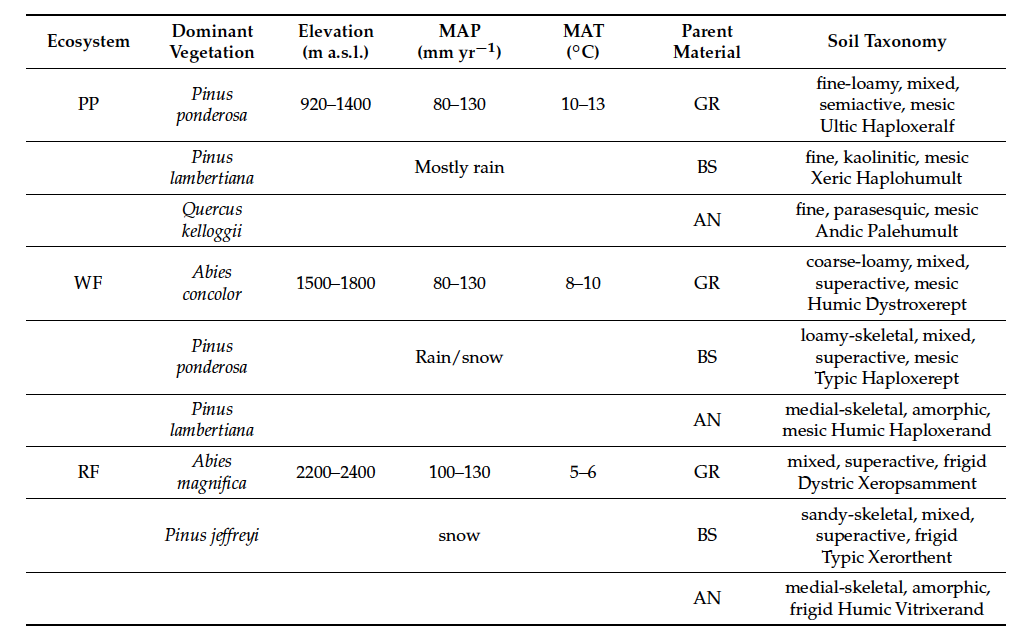
\includegraphics[width=1\linewidth]{../data/img/exp_design_ras18} 

}

\caption{\emph{NB: this is a placeholder---copied verbatim from Rasmussen et al.~2018} Dominant vegetation, climate parameters, and soil taxonomy for sampled ecosystems.\textsuperscript{1} MAP---mean annual precipitation; MAT---Ecosystem abbreviations: PP---ponderosa pine; WF---white fir; RF---red fir. Dominant vegetation is listed in order of over-story dominance. Parent material abbreviations: GR---granite;
BS---basalt; AN---andesite.}\label{fig:exp-design-ras18}
\end{figure}

\hypertarget{sample-collection}{%
\subsection{Sample collection}\label{sample-collection}}

Site locations were initially established in 2001 by C. Rasmussen (Rasmussen et al., 2006), and resampled in 2009 (Rasmussen et al., 2018). We returned in late September of 2019 to collect samples for a third timepoint. Sites were located using GPS and geospatial coordinates recorded during site establishment. At each site we dug three replicate pits down to a depth of 0.3m. Prior to sample collection we compared the soil profiles to the pedon descriptions from the previous sampling campaigns. After confirming profiles were comparable we collected samples from the pit sidewalls in 0.1m increments for each of the three pits. We also measured the depth of the litter layer and collected representative litter samples from each site.

\hypertarget{spline-fitting}{%
\subsection{Spline fitting}\label{spline-fitting}}

Soils collected in 2001 and 2009 were sampled by horizon, while soils collected in 2019 were sampled by depth. We were motivated to use consistent depth increments across sites because of the strong correlation between depth and \(\Delta\)\textsuperscript{14}C. In order to make the horizon and depth-based measurements comparable, we fit a mass-preserving quadratic spline to the 2001 and 2009 profiles in order to convert soil property data to the equivalent depth increments sampled in 2019 (Bishop et al., 2001). We used the mpspline function of the GSIF package in R, with a \(\lambda\) value of 0.1 (Hengl 2019).

\hypertarget{incubations}{%
\subsection{Incubations}\label{incubations}}

Laboratory soil incubations were performed on composite samples from the three replicate pedons sampled at each site in 2001 and 2019. We omitted the 2009 samples from the incubation experiment to save on time and analysis costs. We composited and incubated each depth increment (0-10 cm, 10-20 cm, 20-30 cm) separately in 1 L glass mason jars fitted with sampling ports in the lids. Incubations were performed in duplicate. Prior to the start of incubations we adjusted the soil moisture content to 60\% of water holding capacity (WHC). Samples from 2001 were air-dried prior to archiving, and therefore we also air-dried the freshly collected soils from 2019 in order to control for the known effects of drying and rewetting on \(\Delta\)\textsuperscript{14}C\textsubscript{\emph{respired}} (Beem-Miller et al., 2021). We defined WHC as the gravimetric water content of water-saturated soil placed in mesh-covered (50µm) tubes (50ml) weighed after draining for 30 minutes on a bed of fine sand. Following rewetting we allowed the soils to respire for one week before closing the jars. Incubations proceeded until CO\textsubscript{2} concentrations in the jar headspace reached approximately 10,000 ppm, at which point we collected a 400ml gas subsample for radicocarbon analysis. Gas samples were collected with pre-evacuated stainless-steel (Restec) vacuum canisters. All incubations were performed in the dark at 20°C.

\hypertarget{soil-physical-analyses-and-mineral-characterization}{%
\subsection{Soil Physical Analyses and Mineral Characterization}\label{soil-physical-analyses-and-mineral-characterization}}

Data on soil particle size distributions, bulk density, and mineral characterization were obtained from previously published analyses of samples collected at the study sites in 2001 and 2009 (Rasmussen et al.~2006, Rasmussen et al., 2018). Both qualitative and quantitative approaches were used to characterize soil mineral assemblages, including X-ray diffraction (XRD) for the clay (\textless{}2µm) fraction, atomic absorption spectroscopy, and non-sequential selective dissolution. Details on these analyses are provided by Rasmussen et al. (20XX). In this study we use the sum of ammonium-oxalate extractable aluminum and half of the ammonium-oxalate extractable iron selectively dissolved from bulk soils as a proxy for the abundance of poorly and non-crystalline minerals, and the difference of dithionite-citrate extractable iron and ammonium-oxalate extractable iron for the abundance of crystalline minerals.

\hypertarget{carbon-nitrogen-and-radiocarbon-analysis}{%
\subsection{Carbon, Nitrogen, and Radiocarbon Analysis}\label{carbon-nitrogen-and-radiocarbon-analysis}}

Total carbon and nitrogen content was determined by dry combustion (Vario Max, Elementar Analysensysteme GmbH) on finely ground soils (Retch MM400). For radiocarbon analysis, we first purified CO\textsubscript{2} from incubation flask samples and combusted soil samples on a vacuum line using liquid N\textsubscript{2}. Following purification, samples were graphitized with an iron catalyst under an H\textsubscript{2} enriched atmosphere at 550°C. Radiocarbon content was then measured by accelerator mass spectrometry (Micadas, Ionplus, Switzerland) at the Max Planck Institute for Biogeochemisty (Steinhof, 2017).

We report radiocarbon values using units of \(\Delta\)\textsuperscript{14}C, defined as the deviation in parts per thousand of the ratio of \textsuperscript{14}C--\textsuperscript{12}C from that of the oxalic acid standard measured in 1950. This unit also contains a correction for the potential effect of mass-dependent fractionation by normalizing sample \(\delta\)\textsuperscript{13}C to a common \(\delta\)\textsuperscript{13}C value of -25 per mil (Stuiver \& Polach, 1977). Values with \(\Delta\)\textsuperscript{14}C \textgreater{}0 indicate the presence of \enquote{bomb} C produced by atmospheric weapons testing in the early 1960s. Values with \(\Delta\)\textsuperscript{14}C \textless{} 0 indicate the influence of radioactive decay of \textsuperscript{14}C, which has a half-life 5730 years.

\hypertarget{statistical-analysis}{%
\subsection{Statistical analysis}\label{statistical-analysis}}

We used a linear modeling approach to assess the relative explanatory power of climate versus parent material on the observed variation in \(\Delta\)\textsuperscript{14}C, as well as potential interactions between these two factors. We constructed separate models for \(\Delta\)\textsuperscript{14}C\textsubscript{\emph{bulk}} and \(\Delta\)\textsuperscript{14}C\textsubscript{\emph{respired}} but with the same equation structure (Eq. 1). For each model we considered the two-way interaction between parent material and climate as well as the three-way interaction with time (\textbf{Eq. 1}). For ease of interpretation, we considered the effect of depth by modeling each depth layer separately (0-10 cm, 10-20 cm, 20-30 cm). We also made pairwise comparisons of \(\Delta\)\textsuperscript{14}C\textsubscript{\emph{bulk}} and \(\Delta\)\textsuperscript{14}C\textsubscript{\emph{respired}} across sites and within years, as well as comparisons of individual sites across years. We assessed the significance of the temporal trend for pairwise combinations of parent material and climate using the emmtrends function of the emmeans package (Lenth, 2021). We corrected for multiple comparisons using Tukey's honestly significant mean difference.

\textbf{Eq. 1}
\[\Delta^{14}C = \alpha + \beta_{1}(Parent\_material) \times \beta_{2}(Climate) \times \beta_{3}(Year) + \epsilon\]
The relationship between \(\Delta\)\textsuperscript{14}C of bulk soil and respired CO\textsubscript{2} provides insight into soil C dynamics and potential retention mechanisms (Sierra et al.~2018). We modeled the effects of parent material (\textbf{Eq. 2}) and climate (\textbf{Eq. 3}) on this relationship separately, as we did not have an adequate number of observations to consider the interaction between these two explanatory variables.
We used \(\Delta\)\textsuperscript{14}C measurements made on samples collected in 2001 and 2019, and data from all depths. The three-way interactions of \(\Delta\)\textsuperscript{14}C\textsubscript{\emph{bulk}} and the explanatory variables were not significant with either depth or time for either \textbf{Eq. 3} or \textbf{Eq. 4}, so we did not include those variables in the models.

\textbf{Eq. 2}
\[\Delta^{14}C_{respired} = \alpha + \beta_{1}(\Delta^{14}C_{bulk}) \times \beta_{2}(Parent\_material) + \epsilon\]

\textbf{Eq. 3}
\[\Delta^{14}C_{respired} = \alpha + \beta_{1}(\Delta^{14}C_{bulk}) \times \beta_{2}(Climate) + \epsilon\]

We assessed the relative importance of poorly crystalline versus crystalline iron minerals in protecting soil C from microbial decomposition by regressing \(\Delta\)\textsuperscript{14}C against the concentrations of ammonium-oxalate extractable iron, ammonium-oxalate extractable aluminum, pyrophosphate extractable aluminum, and dithionite-citrate extractable iron (\textbf{Eq. 4}). We fit the model for \(\Delta\)\textsuperscript{14}C\textsubscript{\emph{bulk}}, \(\Delta\)\textsuperscript{14}C\textsubscript{\emph{respired}}, and the difference between \(\Delta\)\textsuperscript{14}C\textsubscript{\emph{respired}} and \(\Delta\)\textsuperscript{14}C\textsubscript{\emph{bulk}} (\(\Delta\)\textsuperscript{14}C\textsubscript{\emph{bulk-respired}}). We used \(\Delta\)\textsuperscript{14}C data from 2001 and 2019. Selective dissolution was only performed for the soils collected in 2001, but were assumed to be comparable for the other time points as these data reflect weathering processes operating at timescales beyond the 18-year duration of this study. We conducted regressions for the entire 0-30 cm depth as extracted metal concentrations did not change substantially by horizon, and this approach allowed us to control for the depth dependence of \(\Delta\)\textsuperscript{14}C as well as simplify interpretation of the data. In order to obtain estimates of these data for the 0-30 cm depth increment we computed carbon mass-weighted means for \(\Delta\)\textsuperscript{14}C\textsubscript{\emph{bulk}} and flux-weighted means for \(\Delta\)\textsuperscript{14}C\textsubscript{\emph{respired}}; these calculations were made prior to determining \(\Delta\)\textsuperscript{14}C\textsubscript{\emph{bulk-respired}}.

\textbf{Eq. 4}
\[\Delta^{14}C = \alpha + \beta_{1}(Metal_{x}) + \beta_{2}(time) + \epsilon\]

\hypertarget{results}{%
\section{Results}\label{results}}

\hypertarget{soil-carbon-concentration-depth-profiles}{%
\subsection{Soil carbon concentration depth profiles}\label{soil-carbon-concentration-depth-profiles}}

We observed both parent material and climate effects on soil C concentration. Carbon concentrations were similar among parent materials for the warm climate sites (\textbf{Fig. \ref{fig:plot-C-profiles}, a}), while at the cool and cold climate sites (\textbf{Fig. \ref{fig:plot-C-profiles}, b, c}) the andesitic soils had higher C concentrations than either the basaltic or granitic soils. The basaltic and granitic soils had similar C concentrations across climate zones, while the cool and cold climate andesitic soils were enriched in C relative to the warm climate soils. Soils showed a similar decrease in C concentration with depth across all sites (\textbf{Fig. \ref{fig:plot-C-profiles}}).

We did not observe significant changes in soil C concentration over time at the majority of sites. However, there were a few exceptions. Most notably, we saw significant increases in soil C concentration for the cold climate andesitic soils at all depths (lower and upper 95\% confidence limits given in brackets), with increases of: 0.20 {[}0.01, 0.40{]}, 0.23 {[}0.12, 0.35{]}, 0.21 {[}0.13, 0.29{]} percent C yr\textsuperscript{-1}, for the 0-10, 10-20, and 20-30 cm depth increments, respectively. We also saw a significant increase in percent C over time for the 10-20cm layer at the warm climate granitic site (0.16 {[}0.05, 0.26{]} percent C yr\textsuperscript{-1}), and significant decreases for the 0-10cm layer at the warm climate andesitic and basaltic sites (-0.19 {[}-0.37, -0.01{]}, 0.04 {[}-0.07, 0.14{]} percent C yr\textsuperscript{-1}). However, since we did not measure bulk density in 2019, we are limited in our assessment of soil carbon stock changes over time (Schrumpf et al., 2013; others?).



\begin{figure}

{\centering 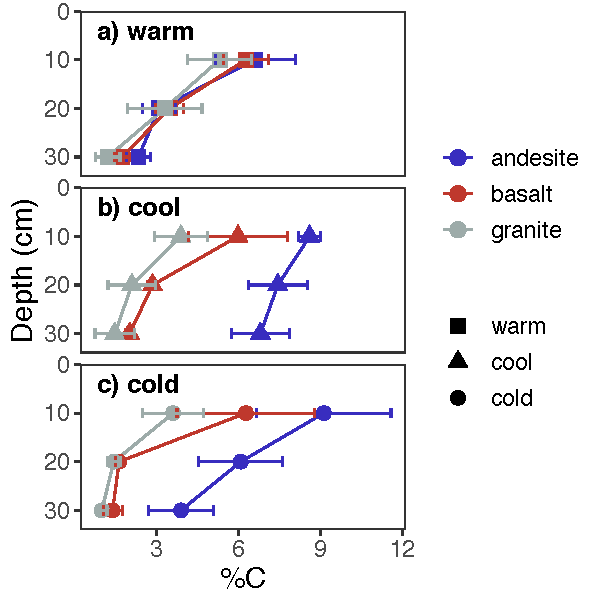
\includegraphics[width=0.65\linewidth,height=0.65\textheight]{sra-blk-inc-19_files/figure-latex/plot-C-profiles-1} 

}

\caption{Profiles of soil C concentration. Points show means of 2001, 2009, and 2019 data; error bars show ±2SE.}\label{fig:plot-C-profiles}
\end{figure}

\hypertarget{radiocarbon-depth-profiles}{%
\subsection{Radiocarbon depth profiles}\label{radiocarbon-depth-profiles}}

\hypertarget{bulk-soil}{%
\subsubsection{Bulk soil}\label{bulk-soil}}

Both parent material and climate covaried with \(\Delta\)\textsuperscript{14}C\textsubscript{\emph{bulk}}, as with soil C concentration. However, contrary to what would be expected from the decomposition-temperature relationship, \(\Delta\)\textsuperscript{14}C\textsubscript{\emph{bulk}} of soils at the cool climate sites was equally or more depleted than what we observed at the cold climate sites (\textbf{Fig. \ref{fig:blk-inc-pro-19}, b, c}), although we observed the most enriched \(\Delta\)\textsuperscript{14}C\textsubscript{\emph{bulk}} at the warm climate sites (\textbf{Fig. \ref{fig:blk-inc-pro-19}, a}). When comparing \(\Delta\)\textsuperscript{14}C\textsubscript{\emph{bulk}} from different parent materials within a given climate zone, \(\Delta\)\textsuperscript{14}C\textsubscript{\emph{bulk}} of andesitic soils tended to be the most depleted, while the granitic soils tended to be the most enriched (\textbf{Fig. \ref{fig:blk-inc-pro-19}}). We focus on the 2019 data here for simplicity, as for \(\Delta\)\textsuperscript{14}C\textsubscript{\emph{bulk}} profiles showed similar patterns in both 2001 (\textbf{SI Fig. 2}) and 2009 (Rasmussen et al., 2018).

Analysis of variance for \(\Delta\)\textsuperscript{14}C\textsubscript{\emph{bulk}} revealed significant two-way interactions between parent material and climate at all depths (\textbf{Table \ref{tab:models-anova}}). This interaction was evident in the differences in \(\Delta\)\textsuperscript{14}C\textsubscript{\emph{bulk}} that we observed among parent materials within a given climate zone. We observed the greatest differences in \(\Delta\)\textsuperscript{14}C\textsubscript{\emph{bulk}} among parent materials at the warm and cool sites (\textbf{Fig. \ref{fig:blk-inc-pro-19}, a, b}), while \(\Delta\)\textsuperscript{14}C\textsubscript{\emph{bulk}} was similar among parent materials at the coldest sites (\textbf{Fig. \ref{fig:blk-inc-pro-19}, c}). We also found depth to be an important factor influencing the relative importance of climate versus parent material effects on \(\Delta\)\textsuperscript{14}C\textsubscript{\emph{bulk}}. Although \(\Delta\)\textsuperscript{14}C\textsubscript{\emph{bulk}} declined with depth for all sites, climate explained more of the variance in \(\Delta\)\textsuperscript{14}C\textsubscript{\emph{bulk}} in the uppermost soil layer (0-10 cm) whereas parent material explained more in the bottom two layers (10-20 cm, 20-30 cm) (\textbf{Table \ref{tab:models-anova}}).

\hypertarget{heterotrophically-respired-co2}{%
\subsubsection{\texorpdfstring{Heterotrophically respired CO\textsubscript{2}}{Heterotrophically respired CO2}}\label{heterotrophically-respired-co2}}

Flux rates of heterotrophic respiration differed among parent materials and among climate zones. When compared on a carbon basis (mgCO\textsubscript{2} gC\textsuperscript{-1} d\textsuperscript{-1}), flux rates tended to be higher for the andesitic soils than soils from either basaltic or andesitic soils, particularly at depth (\textbf{SI Fig. 1}). The exceptions to this trend were soils from 0-10 cm and 10-20 cm depth increments of the warm sites in 2019, for which the granite and basaltic soils both had higher respiration rates than the andesitic soils, and for all three climate zones in the uppermost depth layer of the 2001 samples (\textbf{SI Fig. 2}). Respiration rates for granitic and basaltic soils tended to decrease along the climate gradient; however, we did not see any clear trend in respiration rates with respect to climate for the andesitic soils (\textbf{SI Fig. 2}).

The patterns we observed in \(\Delta\)\textsuperscript{14}C\textsubscript{\emph{respired}} were similar to those we observed in \(\Delta\)\textsuperscript{14}C\textsubscript{\emph{bulk}} (\textbf{Fig. \ref{fig:blk-inc-pro-19}}). We found climate to be the most significant factor for explaining the variance observed in \(\Delta\)\textsuperscript{14}C\textsubscript{\emph{respired}} for the uppermost soil layer, and parent material to be more important than climate for explaining in \(\Delta\)\textsuperscript{14}C\textsubscript{\emph{respired}} variance at the deepest depth, as with \(\Delta\)\textsuperscript{14}C\textsubscript{bulk}. However, unlike \(\Delta\)\textsuperscript{14}C\textsubscript{\emph{bulk}}, parent material was not significant for explaining the variance in \(\Delta\)\textsuperscript{14}C\textsubscript{\emph{respired}} in the uppermost soil layer (\textbf{Table \ref{tab:models-anova}}). Overall, the two-way interaction between parent material and climate explained more of the variance in \(\Delta\)\textsuperscript{14}C\textsubscript{\emph{respired}} data than in the \(\Delta\)\textsuperscript{14}C\textsubscript{\emph{bulk}} data (\textbf{Table \ref{tab:models-anova}, \(F\) values}).

In general, the effect of climate on \(\Delta\)\textsuperscript{14}C\textsubscript{respired} appeared to be moderated by the effect of parent material. For example, we did not observe significant differences in \(\Delta\)\textsuperscript{14}C\textsubscript{\emph{respired}} among the andesitic soils when compared across climate zones at any depth (SI Table X Tukey results for emm?). In contrast, \(\Delta\)\textsuperscript{14}C\textsubscript{\emph{respired}} for the basaltic and granitic soils diverged substantially between climate zones, particularly for the 10-20 cm and 20-30 cm depth layers (\textbf{Fig. \ref{fig:blk-inc-pro-19}}). Overall, \(\Delta\)\textsuperscript{14}C\textsubscript{\emph{respired}} across sites was most similar at the soil surface, and most divergent at the intermediate depth (10-20 cm) (\textbf{Fig. \ref{fig:blk-inc-pro-19}}).



\begin{figure}

{\centering 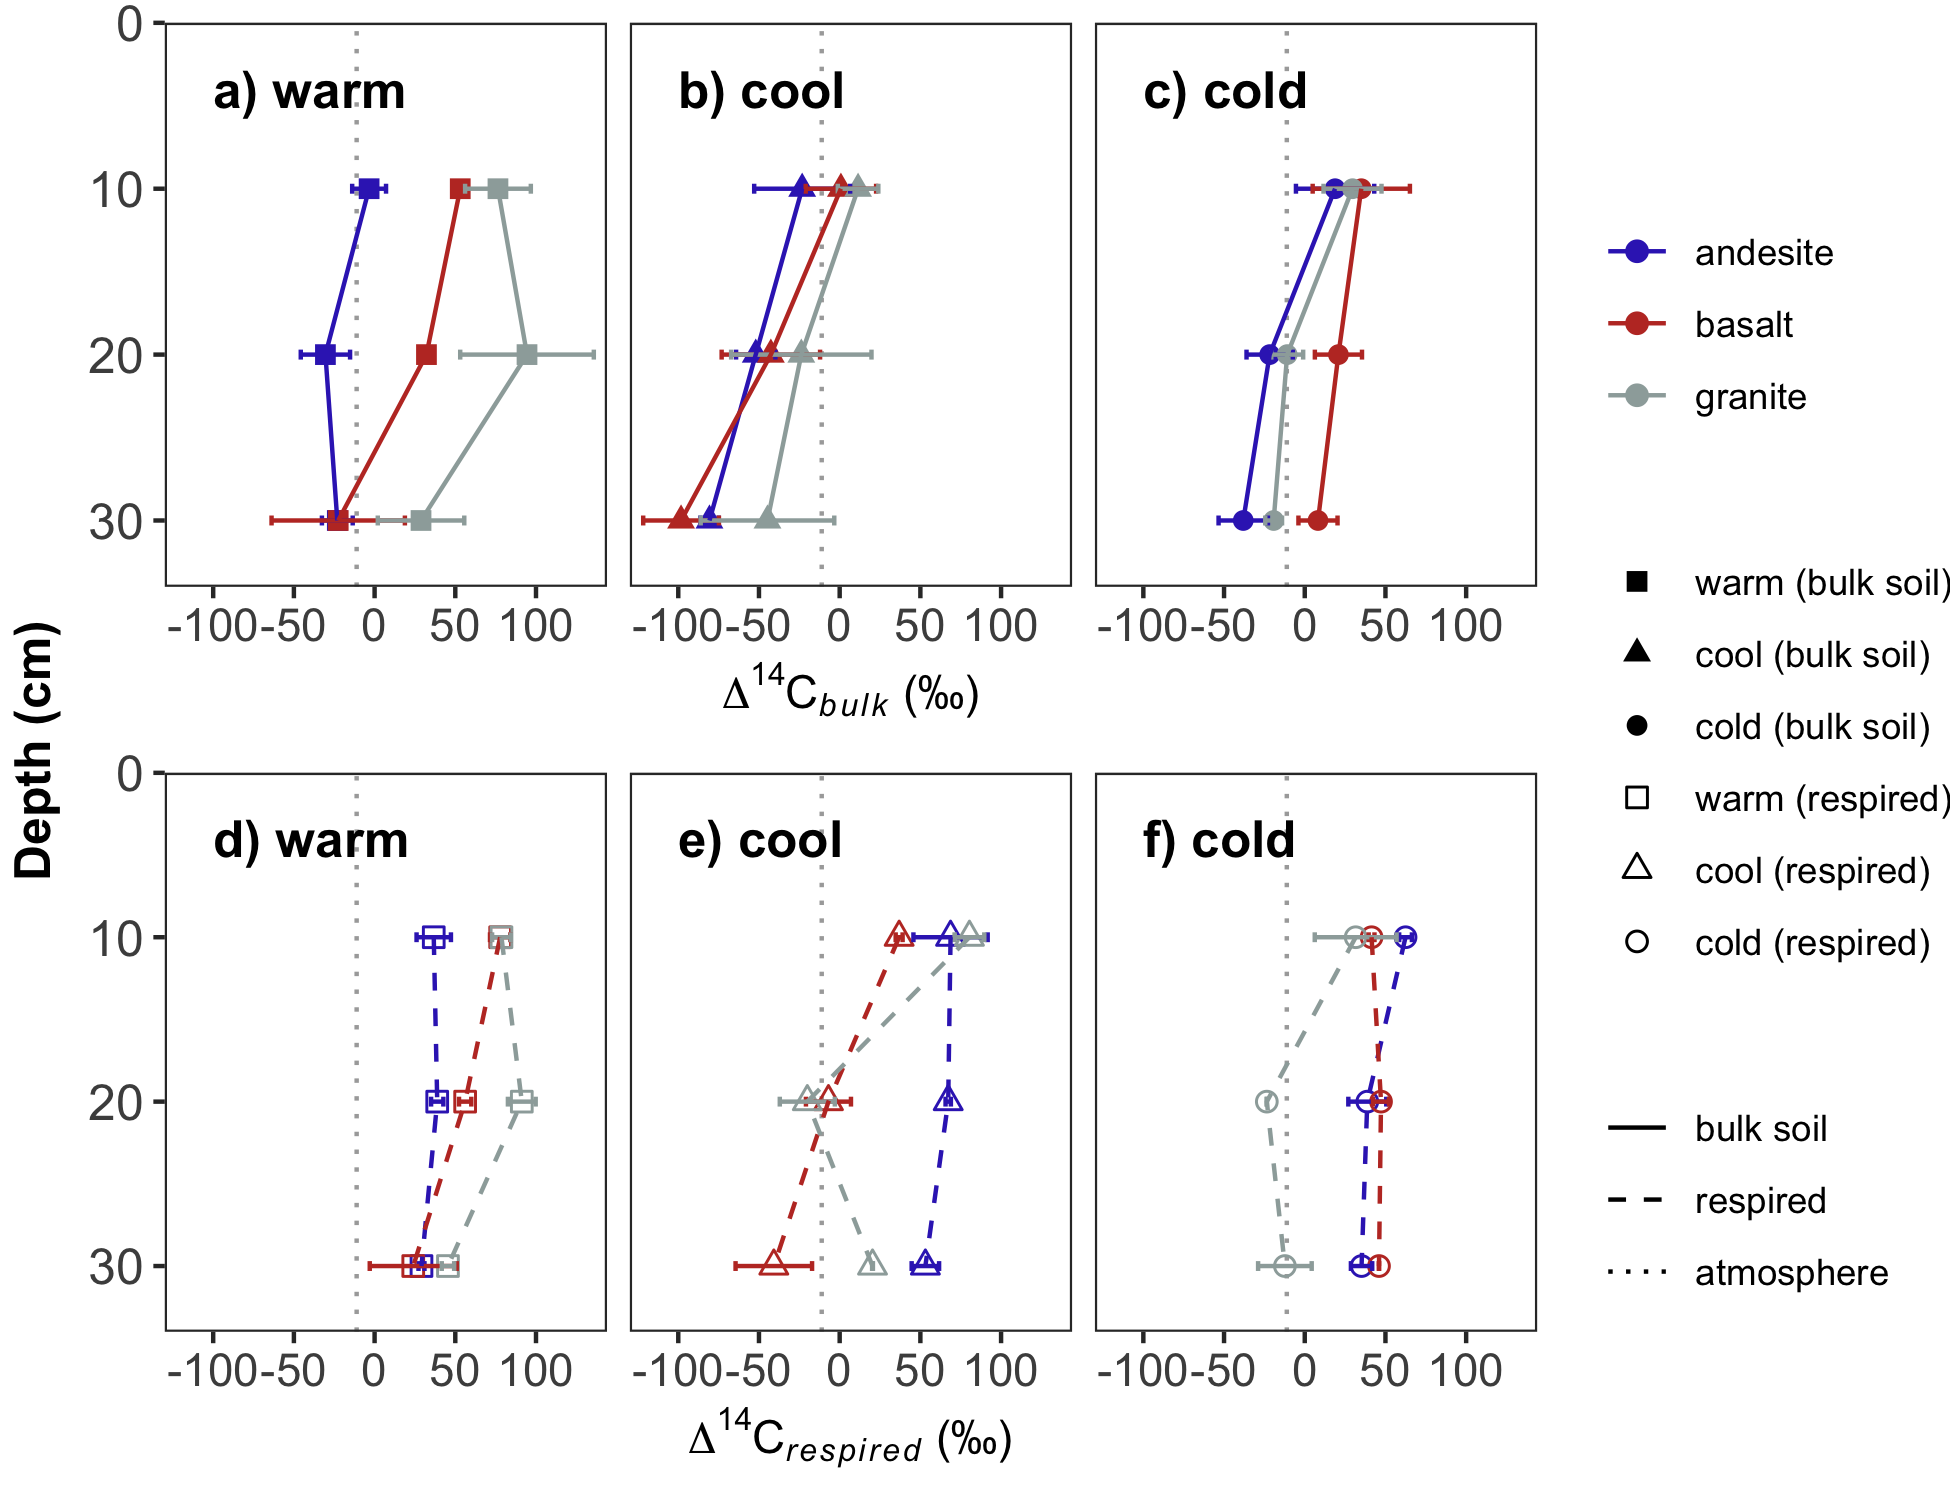
\includegraphics{sra-blk-inc-19_files/figure-latex/blk-inc-pro-19-1} 

}

\caption{Depth profiles of \(\Delta\)\textsuperscript{14}C\textsubscript{\emph{bulk}} and \(\Delta\)\textsuperscript{14}C\textsubscript{\emph{respired}} in 2019. Top panels show bulk data, bottom panels show respired data. Panels (a) and (d) show data from the warm climate sites, (b) and (e) from the cool climate sites, and (c) and (f) from the cold climate sites. Black vertical lines show \(\Delta\)\textsuperscript{14}C of the atmosphere in 2019. Points show the mean of three replicate profiles for bulk soil, and the mean of laboratory duplicates for respired CO\textsubscript{2}. Error bars show ±1 SD for bulk soils and the minimum and maximum for respired CO\textsubscript{2}.}\label{fig:blk-inc-pro-19}
\end{figure}

\hypertarget{radiocarbon-timeseries}{%
\subsection{Radiocarbon timeseries}\label{radiocarbon-timeseries}}

The average annual decline in \(\Delta\)\textsuperscript{14}C atmospheric CO\textsubscript{2} between 2001 and 2009 for the northern hemisphere was -5.13 per mille yr\textsuperscript{-1} (Graven et al., 2017; Sierra, 2018) (\textbf{Fig. \ref{fig:plot-ts-14c}, dotted lines}). Temporal trends in bulk and respired \(\Delta\)\textsuperscript{14}C therefore reflect the degree to which soil C is exchanging with C fixed from the atmosphere. For example, changes in \(\Delta\)\textsuperscript{14}C of soil C that parallel the atmopsheric trend must be exchanging relatively rapidly compared to those that are flat over the same time period.



\begin{figure}

{\centering 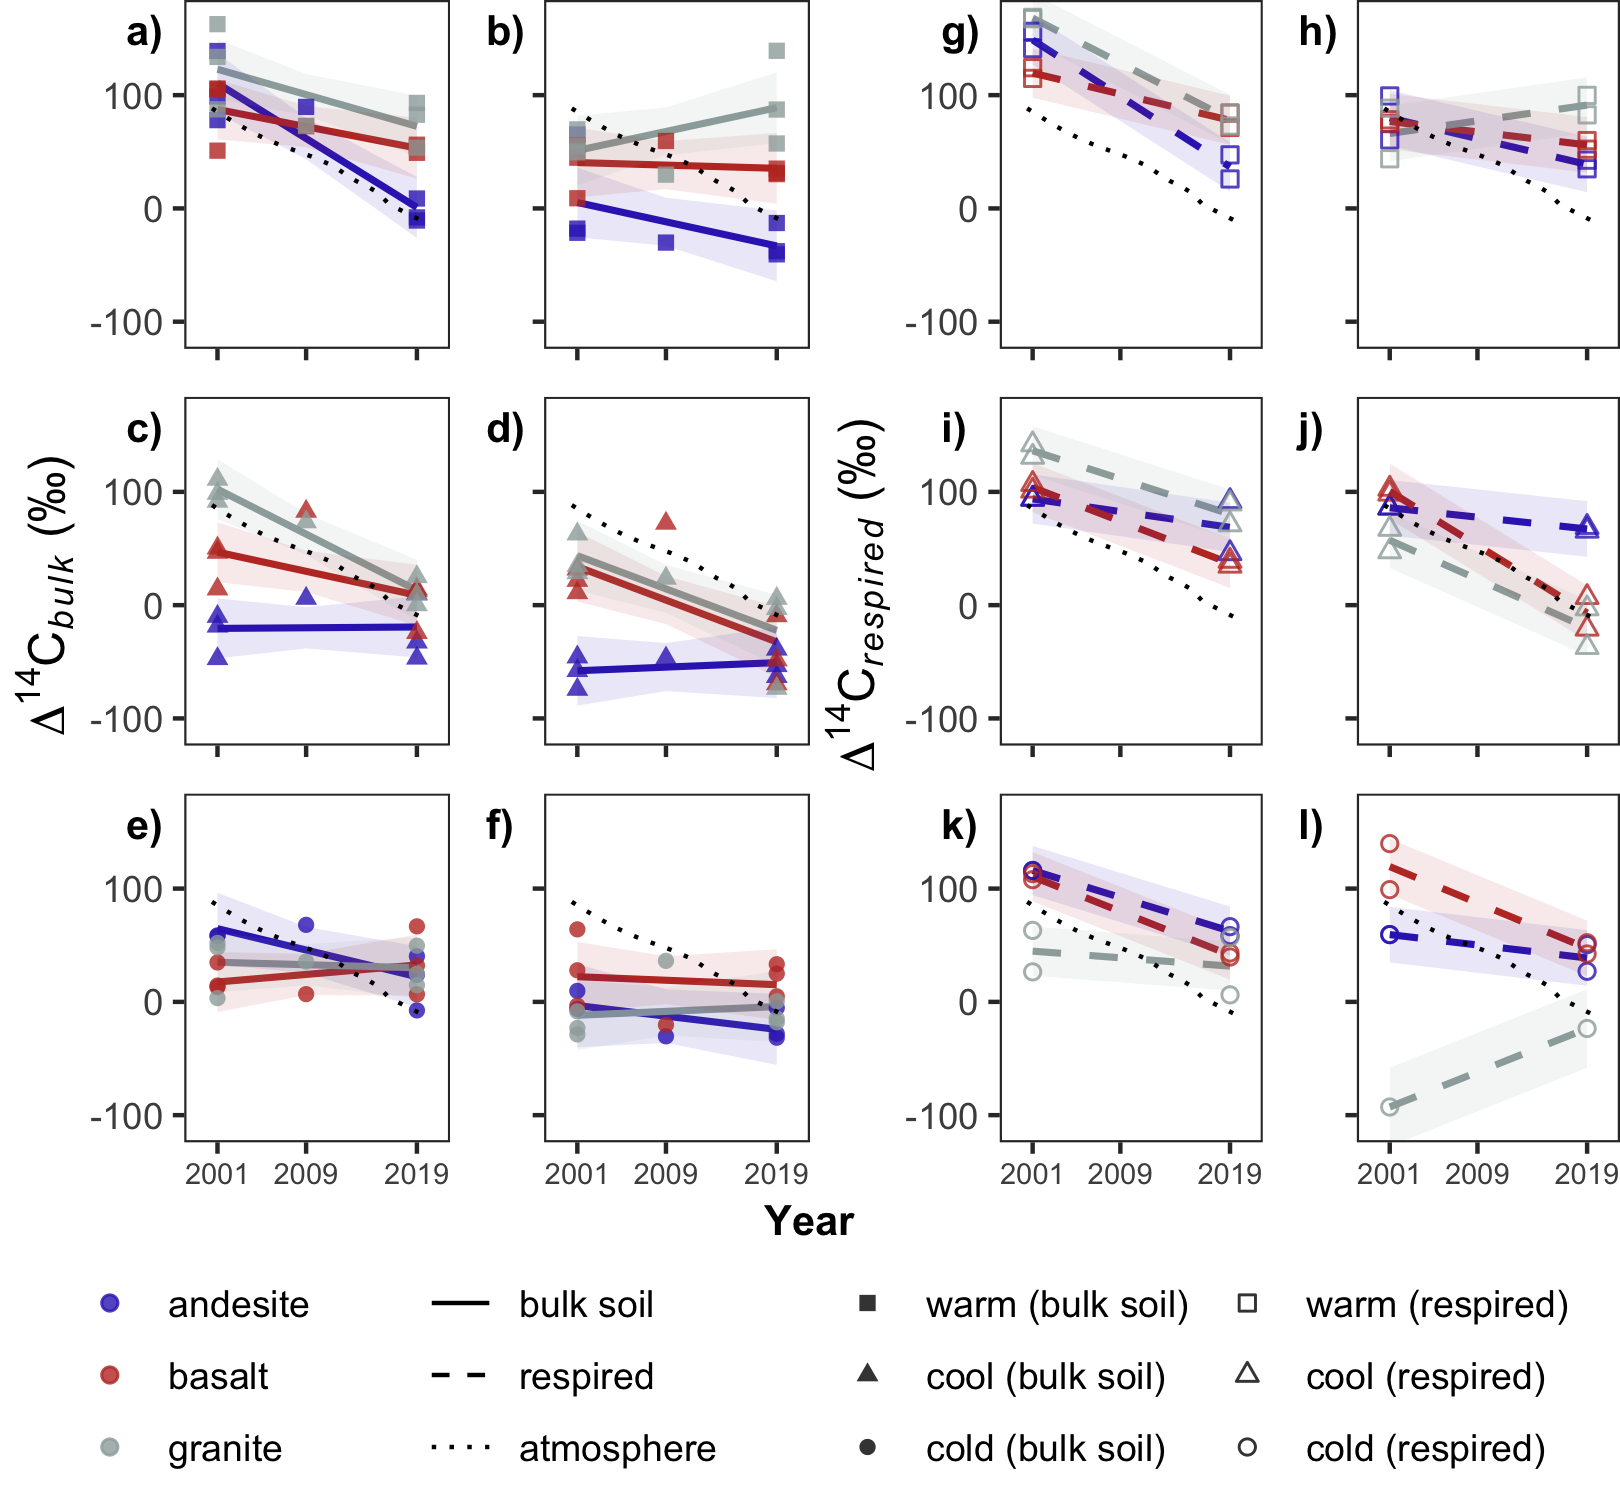
\includegraphics{sra-blk-inc-19_files/figure-latex/plot-ts-14c-1} 

}

\caption{Temporal trends in \(\Delta\)\textsuperscript{14}C for 0-10 cm and 10-20 cm depth layers. Panels a-f show \(\Delta\)\textsuperscript{14}C\textsubscript{\emph{bulk}} data; from left, the first column (panels a, c, and e) show 0-10 cm data, and the second column (panels b, d, and f) shows 10-20 cm data. Panels g-l show \(\Delta\)\textsuperscript{14}C\textsubscript{\emph{respired}} data; the third column from left (panels g, i, k) shows 0-10 cm data, and the rightmost column (panels h, j, and l) shows 10-20 cm data. Points show observed data; lines show linear trend estimates for marginal means; ribbons show 95\% confidence intervals for trends. Dotted line shows atmospheric \(\Delta\)\textsuperscript{14}C.}\label{fig:plot-ts-14c}
\end{figure}



\begingroup\fontsize{10}{12}\selectfont

\begin{longtable}[t]{llrrlrrl}
\caption{\label{tab:models-anova}ANOVA for \(\Delta\)\textsuperscript{14}C\textsubscript{\emph{bulk}} and \(\Delta\)\textsuperscript{14}C\textsubscript{\emph{respired}}}\\
\toprule
\multicolumn{2}{c}{ } & \multicolumn{3}{c}{Bulk soil} & \multicolumn{3}{c}{Respiration} \\
\cmidrule(l{3pt}r{3pt}){3-5} \cmidrule(l{3pt}r{3pt}){6-8}
Depth & Predictor & $df$ & $F$ & $p$ & $df$ & $F$ & $p$\\
\midrule
\endfirsthead
\caption[]{\label{tab:models-anova}ANOVA for \(\Delta\)\textsuperscript{14}C\textsubscript{\emph{bulk}} and \(\Delta\)\textsuperscript{14}C\textsubscript{\emph{respired}} \textit{(continued)}}\\
\toprule
\multicolumn{2}{c}{ } & \multicolumn{3}{c}{Bulk soil} & \multicolumn{3}{c}{Respiration} \\
\cmidrule(l{3pt}r{3pt}){3-5} \cmidrule(l{3pt}r{3pt}){6-8}
Depth & Predictor & $df$ & $F$ & $p$ & $df$ & $F$ & $p$\\
\midrule
\endhead

\endfoot
\bottomrule
\endlastfoot
 & Parent material & 2 & 13.27 & \textbf{< .001} & 2 & 1.03 & 0.377\\
\nopagebreak
 & Climate & 2 & 29.43 & \textbf{< .001} & 2 & 19.28 & \textbf{< .001}\\
\nopagebreak
 & Year & 1 & 33.78 & \textbf{< .001} & 1 & 144.12 & \textbf{< .001}\\
\nopagebreak
 & Parent material:Climate & 4 & 6.38 & \textbf{< .001} & 4 & 12.08 & \textbf{< .001}\\
\nopagebreak
 & Parent material:Year & 2 & 2.43 & 0.1 & 2 & 0.40 & 0.673\\
\nopagebreak
 & Climate:Year & 2 & 5.93 & \textbf{0.005} & 2 & 5.37 & \textbf{0.015}\\
\nopagebreak
 & Parent material:Climate:Year & 4 & 4.67 & \textbf{0.003} & 4 & 5.86 & \textbf{0.003}\\
\nopagebreak
\multirow[t]{-8}{*}{\raggedright\arraybackslash 0-10cm} & Residuals & 44 &  &  & 18 &  & \\
\cmidrule{1-8}\pagebreak[0]
 & Parent material & 2 & 18.53 & \textbf{< .001} & 2 & 6.75 & \textbf{0.007}\\
\nopagebreak
 & Climate & 2 & 8.62 & \textbf{< .001} & 2 & 1.91 & 0.18\\
\nopagebreak
 & Year & 1 & 3.75 & 0.059 & 1 & 0.25 & 0.624\\
\nopagebreak
 & Parent material:Climate & 4 & 1.79 & 0.148 & 4 & 7.01 & \textbf{0.002}\\
\nopagebreak
 & Parent material:Year & 2 & 3.04 & 0.058 & 2 & 10.56 & \textbf{0.001}\\
\nopagebreak
 & Climate:Year & 2 & 9.28 & \textbf{< .001} & 2 & 7.61 & \textbf{0.005}\\
\nopagebreak
 & Parent material:Climate:Year & 4 & 2.62 & \textbf{0.048} & 4 & 2.29 & 0.104\\
\nopagebreak
\multirow[t]{-8}{*}{\raggedright\arraybackslash 20-30cm} & Residuals & 44 &  &  & 16 &  & \\*
\end{longtable}
\endgroup{}

\hypertarget{bulk-soil-1}{%
\subsubsection{Bulk soil}\label{bulk-soil-1}}

We observed a significant three-way interaction between parent material, climate, and time at all three depths in the linear models (\textbf{Eq. 1}) for \(\Delta\)\textsuperscript{14}C\textsubscript{\emph{bulk}} (\textbf{Table \ref{tab:models-anova}}). The change over time in \(\Delta\)\textsuperscript{14}C\textsubscript{\emph{bulk}} was also affected by depth, with greater differences between 2001 and 2019 seen in the uppermost soil layer than in the deeper layers (\textbf{Fig. \ref{fig:plot-ts-14c}}). We observed a significant decrease in \(\Delta\)\textsuperscript{14}C\textsubscript{\emph{bulk}} in both warm and cool climate granitic soils for the uppermost soil layer, and additionally for the warm climate andesitic soils (\textbf{Fig. \ref{fig:plot-ts-14c}, a}). In the deeper soil layers (10-20 cm and 20-30 cm), we only observed a significant change over time in \(\Delta\)\textsuperscript{14}C\textsubscript{\emph{bulk}} in the cool climate basalt and granite soils (\textbf{Fig. \ref{fig:plot-ts-14c}, b, c}). \(\Delta\)\textsuperscript{14}C\textsubscript{\emph{bulk}} of the cool climate andesitic soils remained essentially unchanged between 2001 and 2019 for all depths (\textbf{Fig. \ref{fig:plot-ts-14c}, a, b, c}), underscoring the importance of the interaction between parent material and climate for explaining temporal trends in \(\Delta\)\textsuperscript{14}C\textsubscript{\emph{bulk}} as well as variance in a given year.

The relationship of \(\Delta\)\textsuperscript{14}C\textsubscript{\emph{bulk}} to atmospheric \(\Delta\)\textsuperscript{14}C also depended on the combination of parent material and climate. In 2001, the warm climate sites were the only sites where the basaltic and andesitic soils were enriched relative to the atmosphere, and this enrichment was only observed for the uppermost soil layer (\textbf{Fig. \ref{fig:plot-ts-14c})}). In contrast, granitic soils at both the warm and cool granitic sites were enriched relative to the atmosphere in 2001 (\textbf{Fig. \ref{fig:plot-ts-14c}}). For the cold climate sites, where \(\Delta\)\textsuperscript{14}C\textsubscript{\emph{bulk}} was most similar, all three lithologies were depleted relative to atmospheric in both surface and subsoil layers (\textbf{Fig. \ref{fig:plot-ts-14c}}).

We observed that \(\Delta\)\textsuperscript{14}C\textsubscript{\emph{bulk}} tended to decrease or remain unchanged between 2001 and 2019 across sites, but the rates of change in \(\Delta\)\textsuperscript{14}C\textsubscript{\emph{bulk}} were typically smaller than the corresponding change in atmospheric \(\Delta\)\textsuperscript{14}C over the same period. Accordingly, \(\Delta\)\textsuperscript{14}C\textsubscript{\emph{bulk}} measured in 2019 tended to be enriched relative to the atmosphere at more sites, and also deeper into the soil than in 2001. We observed surface soil \(\Delta\)\textsuperscript{14}C\textsubscript{\emph{bulk}} (0-10 cm) in 2019 to be enriched relative to the atmosphere at all sites except for the cool climate andesite soils (\textbf{Fig. \ref{fig:plot-ts-14c}; Fig. \ref{fig:blk-inc-pro-19}, d-f}). Furthermore, \(\Delta\)\textsuperscript{14}C\textsubscript{\emph{bulk}} remained enriched relative to the atmosphere down to 30 cm at two of the sites in 2019: the warm climate granite soil (\textbf{Fig. \ref{fig:blk-inc-pro-19}, d}) and cold climate basalt soil (\textbf{Fig. \ref{fig:blk-inc-pro-19}, f}). \(\Delta\)\textsuperscript{14}C\textsubscript{\emph{bulk}} at the cool andesite site was the most depleted relative to the atmosphere at all time points (\textbf{Fig. \ref{fig:plot-ts-14c}}).

\hypertarget{heterotrophically-respired-co2-1}{%
\subsubsection{\texorpdfstring{Heterotrophically respired CO\textsubscript{2}}{Heterotrophically respired CO2}}\label{heterotrophically-respired-co2-1}}

Temporal trends in \(\Delta\)\textsuperscript{14}C\textsubscript{\emph{respired}} were similar to what we observed for \(\Delta\)\textsuperscript{14}C\textsubscript{\emph{bulk}}, but tended to be of greater magnitude (\textbf{Fig. \ref{fig:plot-ts-14c}, g-l}). Although greater than the change over time we observed in \(\Delta\)\textsuperscript{14}C\textsubscript{\emph{bulk}}, changes in \(\Delta\)\textsuperscript{14}C\textsubscript{\emph{respired}} between 2001 and 2019 still tended to be smaller in magnitude than the change observed in the atmosphere over this period (\textbf{Fig. \ref{fig:plot-ts-14c}, g-l}). In contrast to \(\Delta\)\textsuperscript{14}C\textsubscript{\emph{bulk}}, \(\Delta\)\textsuperscript{14}C\textsubscript{\emph{respired}} tended to be indistinguishable or enriched relative to the atmosphere in both 2001 and 2019; while the majority of samples were enriched relative to the atmosphere in 2019, even at depth (\textbf{Fig. \ref{fig:plot-ts-14c}, g-l}).

We saw significant decreases in surface soil \(\Delta\)\textsuperscript{14}C\textsubscript{\emph{respired}} at seven of the nine sites, with the only exceptions being the cool andesitic and cold granitic sites (\textbf{Fig. \ref{fig:plot-ts-14c}, i, k}). In absolute terms, the changes in \(\Delta\)\textsuperscript{14}C\textsubscript{\emph{respired}} over time in these uppermost soil layers were greatest at the warm sites (-4.5 per mil ±2 yr\textsuperscript{-1}), while changes were similar for the cool and cold sites (-2.7 per mil ±1.2 yr\textsuperscript{-1}, and -2.5 per mil ±1.6 yr\textsuperscript{-1}, respectively). When considered within parent materials, granitic soils showed greatest decreases \(\Delta\)\textsuperscript{14}C\textsubscript{\emph{respired}} over time at the warm climate sites and the least change at the cold climate sites. In contrast, the andesitic soils showed the least amount of change over time at the cool climate sites, while there were no significant differences among climate zones for the basaltic soils. The magnitude of the change in \(\Delta\)\textsuperscript{14}C\textsubscript{\emph{respired}} over time tended to decrease with depth for all soils. We observed significant negative trends over time for \(\Delta\)\textsuperscript{14}C\textsubscript{\emph{respired}} at only four of the nine sites for the 10-20 cm layer (warm andesite, cool basalt, cool granite, and cold basalt) (\textbf{Fig. \ref{fig:plot-ts-14c}}), and only one site for the 20-30 cm layer (cold basalt) (SI). \(\Delta\)\textsuperscript{14}C\textsubscript{\emph{respired}} at the cool andesitic soils remained unchanged at all depths over the study period.

We observed a significant increase in \(\Delta\)\textsuperscript{14}C\textsubscript{\emph{respired}} from 2001 to 2019 at only one site: from the cold climate granitic soils (\textbf{Fig. \ref{fig:plot-ts-14c}}). These were also the only soils for which \(\Delta\)\textsuperscript{14}C\textsubscript{\emph{respired}} was more depleted than \(\Delta\)\textsuperscript{14}C\textsubscript{\emph{bulk}}. We observed this anomaly for the deeper soil layers in both 2001 and 2019. For the 8-27 cm layer in 2001, the range of \(\Delta\)\textsuperscript{14}C\textsubscript{\emph{respired}} values was -469.10 and -127.80 per mil, compared to a range of \(\Delta\)\textsuperscript{14}C\textsubscript{\emph{bulk}} values of -30.80 and -10.50; similarly, for the 10-20 cm layer in 2019 we observed a range of \(\Delta\)\textsuperscript{14}C\textsubscript{\emph{respired}} values of -396.70 and -23.50 per mil compared to -18.10 and 0.40 for \(\Delta\)\textsuperscript{14}C\textsubscript{\emph{bulk}} (SI Table X). We do not believe this was due to laboratory error in spite of the high variance we observed in the samples, as the pattern was restricted to the deeper soil layers from this one site and consistent over time. However, since it appears to be a unique response to these soils, we have excluded these highly depleted samples from the statistical analyses.

\hypertarget{relationship-of-bulk-soil-and-respired-co2-delta14c}{%
\subsection{\texorpdfstring{Relationship of bulk soil and respired CO\textsubscript{2} \(\Delta\)\textsuperscript{14}C}{Relationship of bulk soil and respired CO2 \textbackslash{}Delta14C}}\label{relationship-of-bulk-soil-and-respired-co2-delta14c}}

We assessed the relationship between \(\Delta\)\textsuperscript{14}C\textsubscript{\emph{bulk}} and \(\Delta\)\textsuperscript{14}C\textsubscript{\emph{respired}} using linear regression models for parent material (\textbf{Eq. 3}) and climate (\textbf{Eq. 4}). We observed \(\Delta\)\textsuperscript{14}C\textsubscript{\emph{respired}} to be enriched relative to \(\Delta\)\textsuperscript{14}C\textsubscript{\emph{bulk}} for almost all sites and all depths, but that the magnitude of the difference depended on both parent material and climate. Accordingly, we found that all of the models had y-intercept equal to or greater than zero for all parent materials and all climate zones, indicating that respired CO\textsuperscript{2} in these soils is predominantly modern (i.e. \textless{} 60 years old) for all but the deepest soil layers. We found the largest y-intercept values for the soils developed on andesitic parent material and for soils in the cool climate zones, showing that these soils are relatively enriched in decadally cycling bomb-C.

Slope values less than 1 in these models indicate that the process or processes leading to greater bulk soil C ages leads to a correspondigly smaller decrease in the age of respired CO\textsubscript{2}. Similar to what we found for the y-intercepts, modeled slopes for the parent material only model were smallest for the andesitic soils (slope = 0.51, 95\% CI = {[}0.22, 0.80{]}) (\textbf{Fig. \ref{fig:blk-inc-plots}, a}), and for cool climate soils in the climate only model (\textbf{Eq. 3}) (slope = 0.61, 95\% CI = {[}0.30, 0.91{]}) (\textbf{Fig. \ref{fig:blk-inc-plots}, b}). While we could not directly test the interaction of parent material and climate factors in these models owing to the limited number of observations, we observed that mean differences in \(\Delta\)\textsuperscript{14}C\textsubscript{\emph{bulk}} and \(\Delta\)\textsuperscript{14}C\textsubscript{\emph{respired}} were substantially greater for the cool climate soils developed on andesitic parent material than for the other sites.



\begin{figure}

{\centering 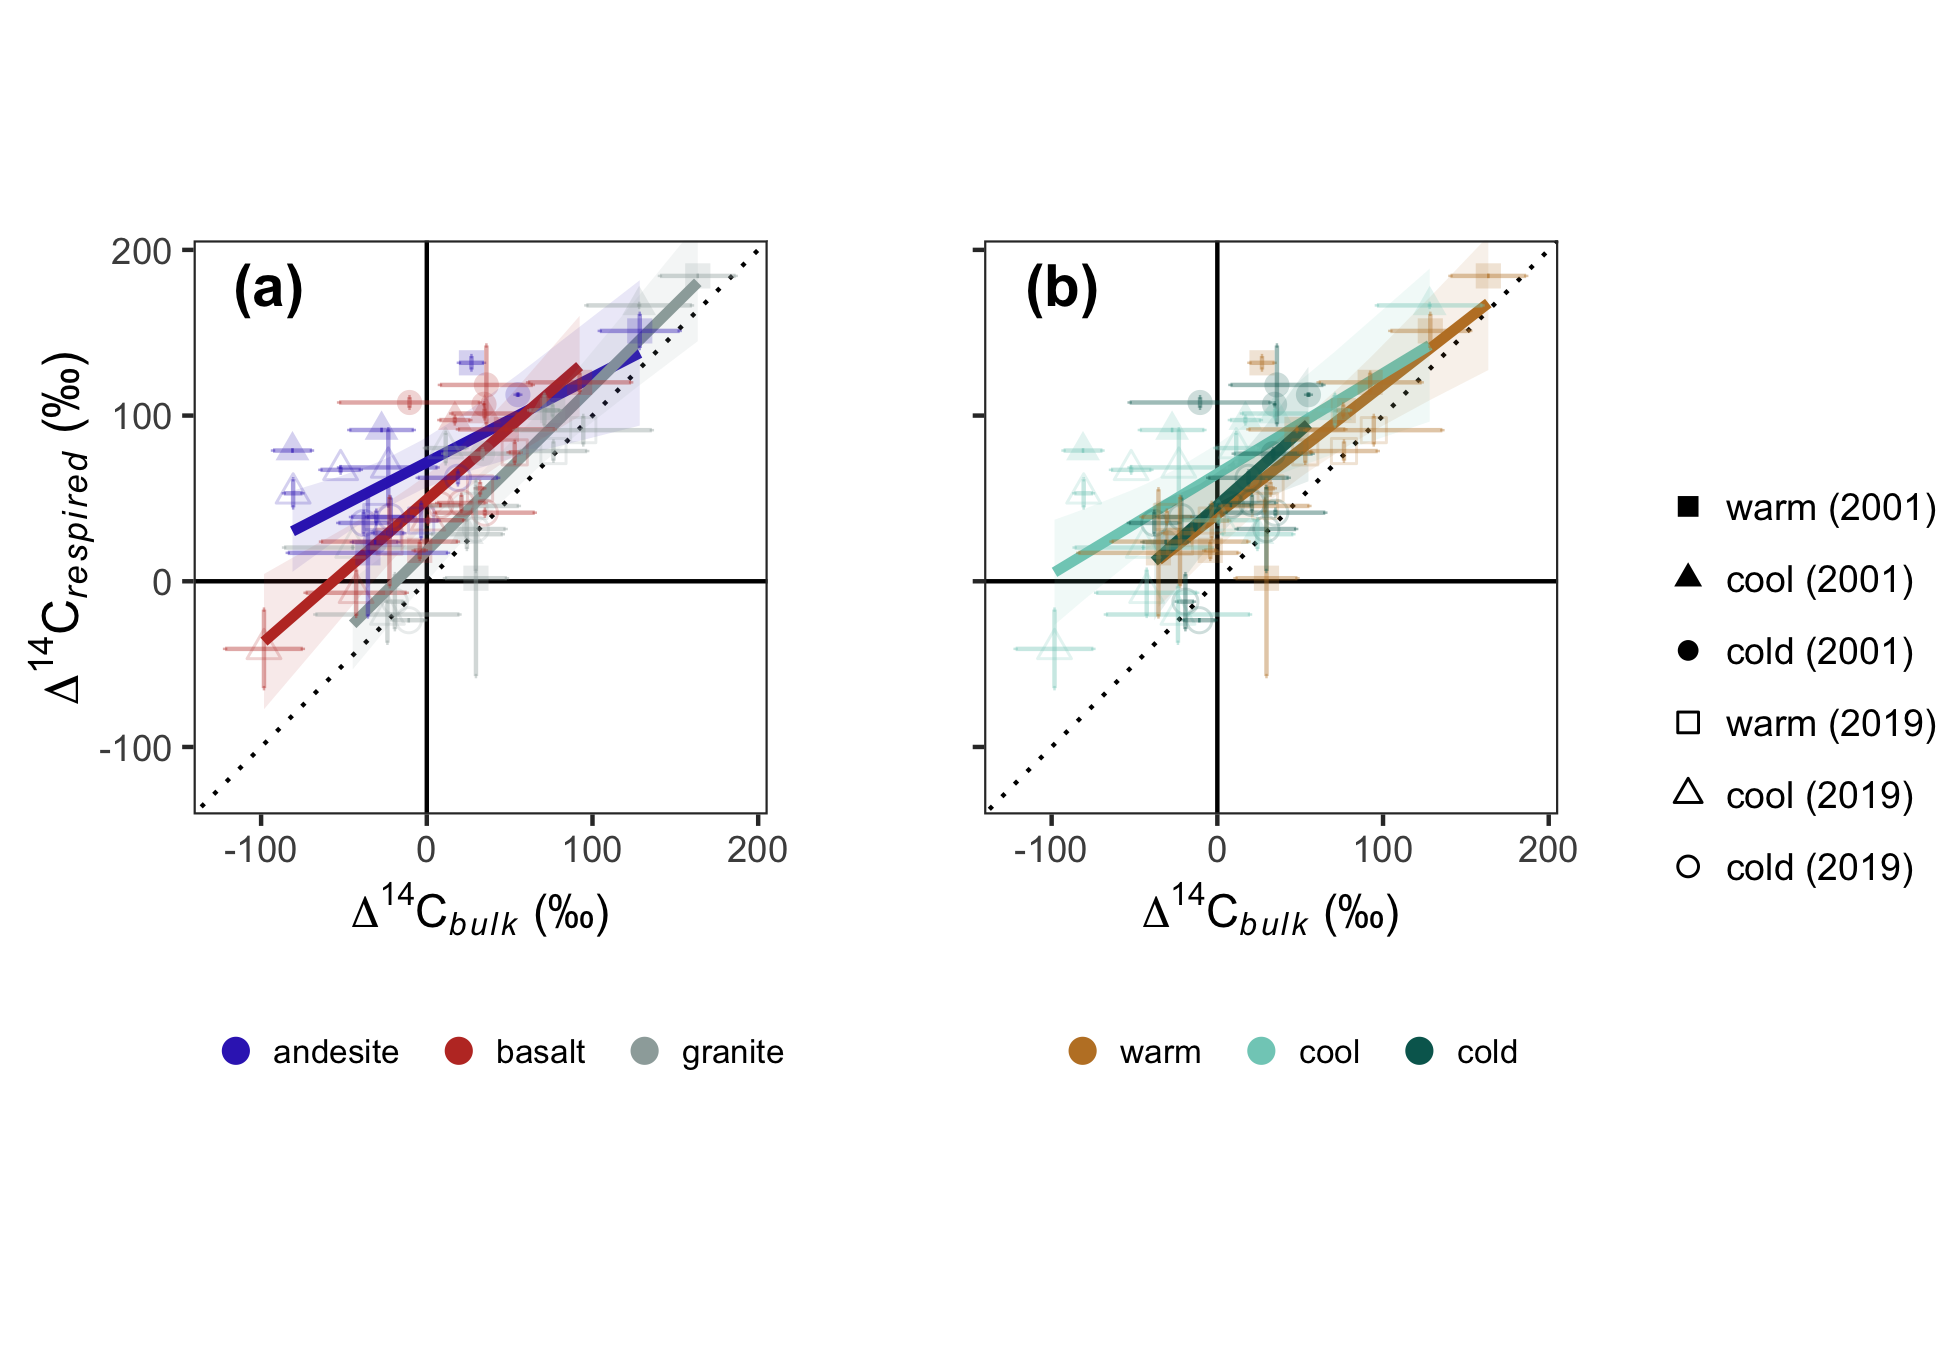
\includegraphics{sra-blk-inc-19_files/figure-latex/blk-inc-plots-1} 

}

\caption{Parent material and climate effects on the relationship of \(\Delta\)\textsuperscript{14}C\textsubscript{\emph{bulk}} and \(\Delta\)\textsuperscript{14}C\textsubscript{\emph{respired}}. \textsuperscript{a)} Parent material model \textbf{(Eq. 3)} and \textsuperscript{b)} Climate model \textbf{(Eq. 4)}. Dotted line shows 1:1 relationship. Points show the mean of three replicate profiles for bulk soil, and the mean of laboratory duplicates for respired CO\textsubscript{2}. Error bars show ±1 SD for bulk soils and the minimum and maximum for respired CO\textsubscript{2}. Respired CO\textsubscript{2} from the cold granite site in 2001 was extremely depleted in \(\Delta\)\textsuperscript{14}C and thus is excluded for display purposes.}\label{fig:blk-inc-plots}
\end{figure}

\hypertarget{mineral-assemblages-and-radiocarbon}{%
\subsection{Mineral assemblages and radiocarbon}\label{mineral-assemblages-and-radiocarbon}}

Mineral assemblage data is reported fully in Rasmussen et al. (2018). Here we focus on the selective dissolution data with respect to the trends we observed in \(\Delta\)\textsuperscript{14}C\textsubscript{\emph{bulk}}, \(\Delta\)\textsuperscript{14}C\textsubscript{\emph{respired}}, and \(\Delta\)\textsuperscript{14}C\textsubscript{\emph{respired-bulk}}. We observed a significant negative correlation between \(\Delta\)\textsuperscript{14}C\textsubscript{\emph{bulk}} and the concentration of oxalate extractable iron, oxalate extractable aluminum, and pyrophosphate extractable aluminum (SI). For simplicity, we focus here on the sum of oxalate extractable aluminum and half of the oxalate extractable iron as a proxy for poorly crystalline mineral abundance, and the difference of dithionite-citrate extractable iron and ammonium-oxalate extractable iron as a proxy for crystalline mineral abundance. The relationship between non-crystalline mineral abundance and \(\Delta\)\textsuperscript{14}C\textsubscript{\emph{bulk}} was highly significant (\emph{p} \textless{}0.001), with the model explaining 56.00 percent of the observed variation. In contrast, we did not find a significant relationship between crystalline mineral abundance and \(\Delta\)\textsuperscript{14}C\textsubscript{\emph{bulk}}.

We also observed a significant (\emph{p} = 0.02) negative relationship between \(\Delta\)\textsuperscript{14}C\textsubscript{\emph{respired}} and non-crystalline mineral abundance, although it was not as strong as the \(\Delta\)\textsuperscript{14}C\textsubscript{\emph{bulk}} relationship. However, we observed a stronger relationship between poorly crystalline mineral abundance and \(\Delta\)\textsuperscript{14}C\textsubscript{\emph{respired-bulk}} (\textbf{Fig. \ref{fig:plot-min-14c-0-30-blk-inc}, a}) than for either \(\Delta\)\textsuperscript{14}C\textsubscript{\emph{bulk}} or \(\Delta\)\textsuperscript{14}C\textsubscript{\emph{respired}}. As with \(\Delta\)\textsuperscript{14}C\textsubscript{\emph{bulk}}, there was no relationship with crystalline mineral abundance for either \(\Delta\)\textsuperscript{14}C\textsubscript{\emph{bulk}} or \(\Delta\)\textsuperscript{14}C\textsubscript{\emph{respired-bulk}} (\textbf{Fig. \ref{fig:plot-min-14c-0-30-blk-inc}, b}).



\begin{figure}

{\centering 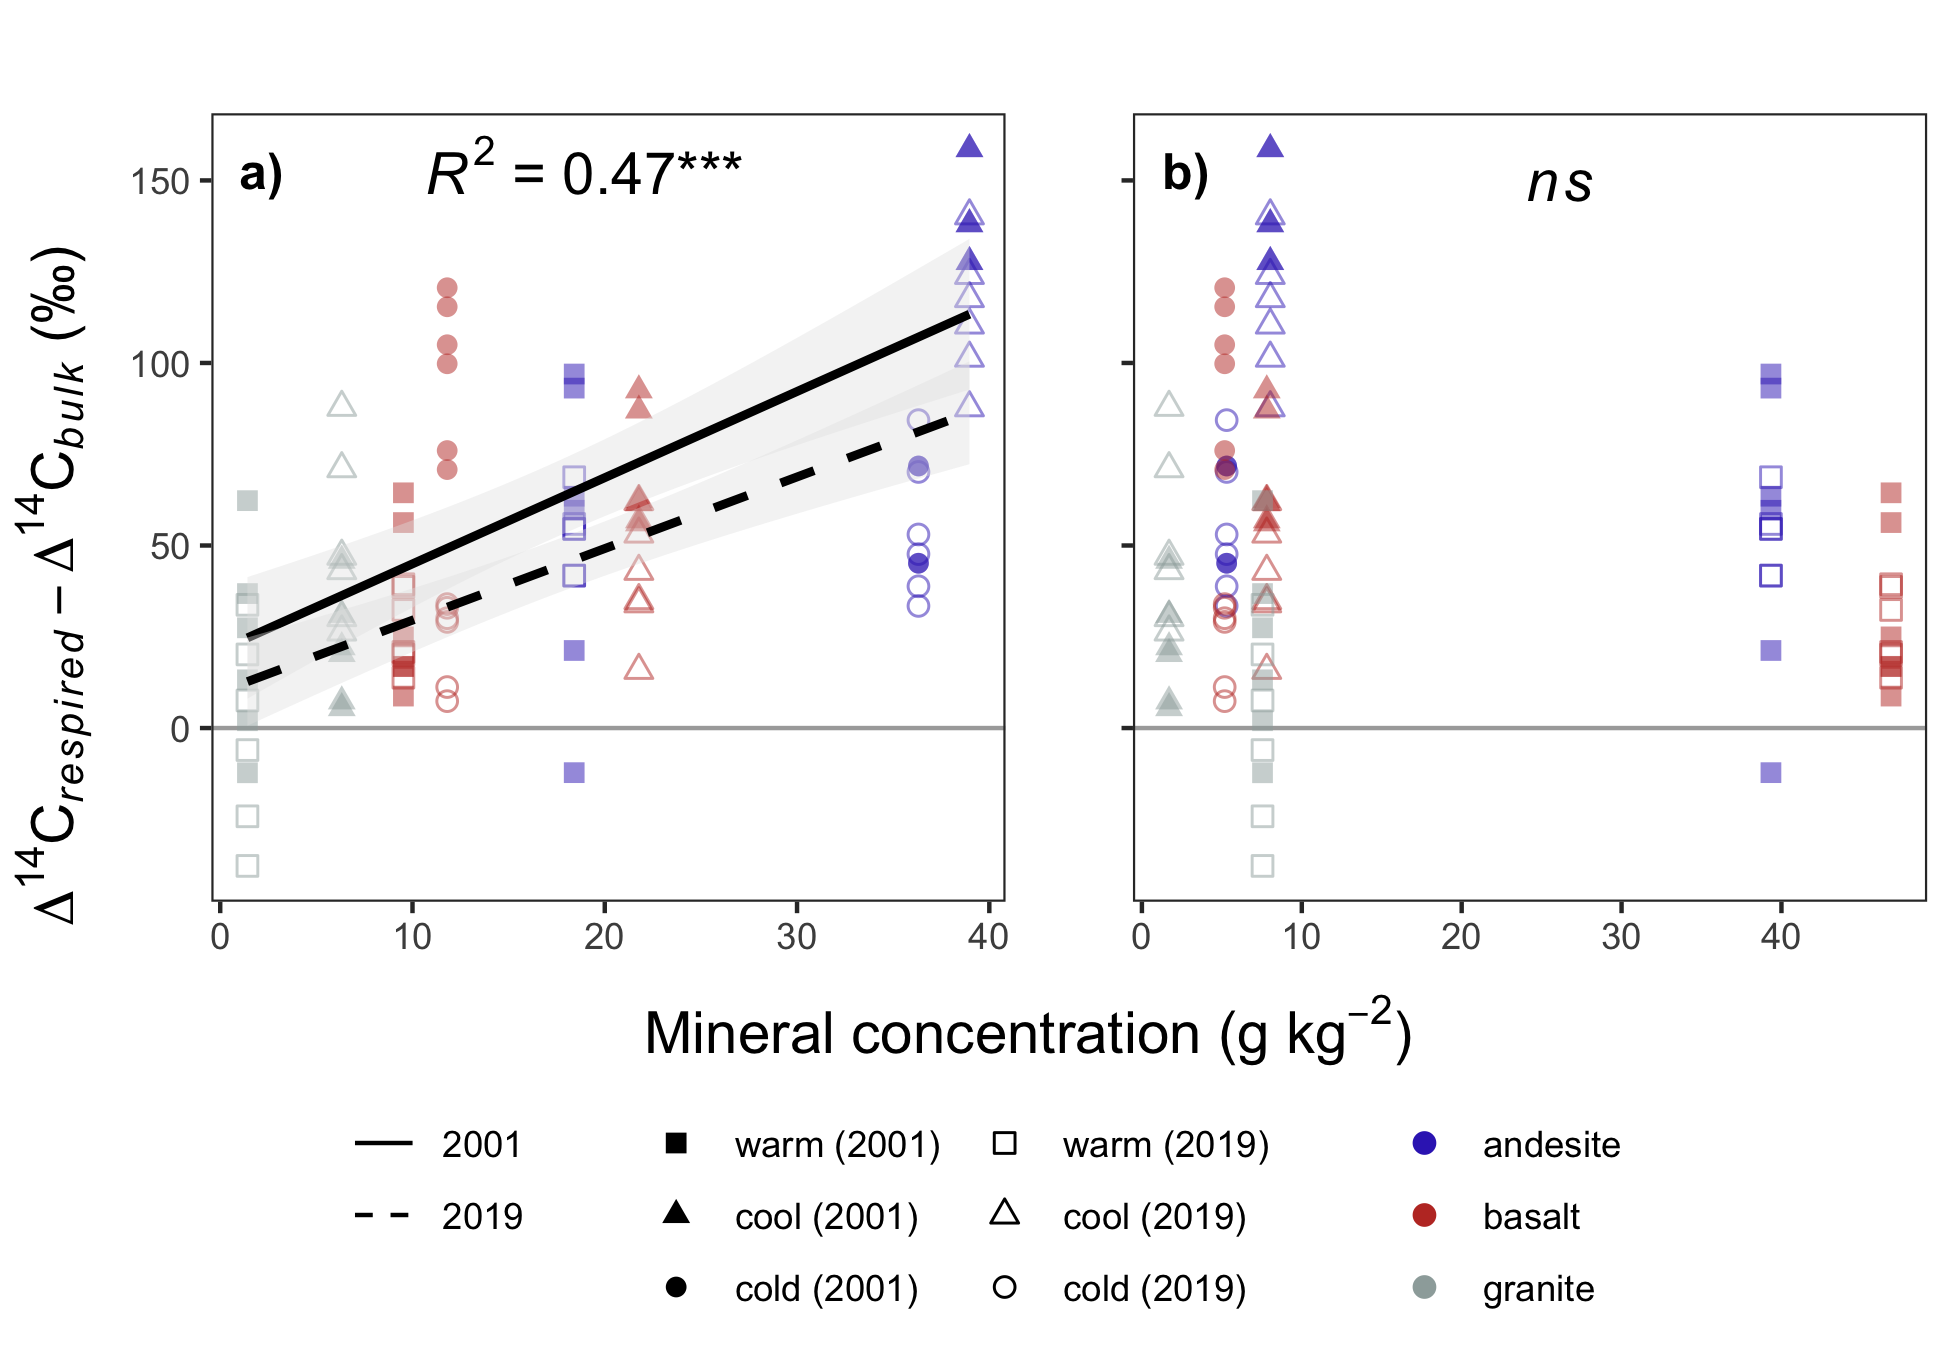
\includegraphics{sra-blk-inc-19_files/figure-latex/plot-min-14c-0-30-blk-inc-1} 

}

\caption{Relationship of poorly crystalline and crystalline minerals to the difference of \(\Delta\)\textsuperscript{14}C\textsubscript{\emph{respired}} and \(\Delta\)\textsuperscript{14}C\textsubscript{\emph{bulk}} (\(\Delta\)\textsuperscript{14}C\textsubscript{\emph{respired-bulk}}). \textsuperscript{a)} Poorly crystalline mineral content (oxalate-extractable aluminum + 1/2 oxalate-extractable iron), \textsuperscript{b)} Crystalline mineral content (dithionite-extractable iron - oxalate-extractable iron). Points show mass-weighted mineral concentrations and carbon-weighted values of \(\Delta\)\textsuperscript{14}C\textsubscript{\emph{respired-bulk}} for 0-30cm profiles. Lines show linear model fits from \textbf{Eq. 5}.}\label{fig:plot-min-14c-0-30-blk-inc}
\end{figure}

\hypertarget{discussion}{%
\section{Discussion}\label{discussion}}

Climate and the association of soil organic matter with minerals play key roles in soil organic persistence. However, the relevance of parent material for explaining soil organic matter persistence in soils with mixed mineralogies is still poorly explained. In the current study we illuminate how parent material interactions with climate via weathering lead to the development of distinct mineral assemblages, which in turn control the dynamics of soil C cycling at timescales ranging from annual to centennial. Our key finding is that soil mineral characteristics mediate climatic controls on soil C cycling, and that mineralogical controls on soil C cycling are not limited to soil C persistence on centennial timescales, but are also relevant for C cycling on shorter timescales as well.

Our results challenge the primacy of climate control on soil carbon persistence, insofar as we observed the most depleted \(\Delta\)\textsuperscript{14}C\textsubscript{\emph{bulk}} in soils of the cool climate zone, not the cold climate zone. We found that climate is still a critical factor for explaining the dynamics of both persistent and more transient soil C pools, as measured by proxy with \(\Delta\)\textsuperscript{14}C\textsubscript{\emph{bulk}} and \(\Delta\)\textsuperscript{14}C\textsubscript{\emph{respired}}, respectively, but our results indicate that soil mineral characteristics moderate the strength of the climate effect. This is particularly apparent at depth. These results are supported by a recent study in which the authors used a depth-resolved model with energy and substrate limitation proscribed by Michalis Menten kinetics to model profiles of \(\Delta\)\textsuperscript{14}C\textsubscript{\emph{bulk}} (Ahrens et al.~2020). The authors found that site mean annual temperature could only explain a minimal amount of variation in the observed radiocarbon profiles, while varying sorption potential in the model allowed for a superior fit.

Previous work at our study sites showed that poorly crystalline minerals were key to explaining both soil C accumulation and bulk soil C ages in these soils (Rasmussen et al., 2018). Our results confirm these findings and extend them to demonstrate a significant negative correlation between poorly crystalline mineral content and \(\Delta\)\textsuperscript{14}C\textsubscript{\emph{respired}}. However, the interpretation of this relationship is complicated by the bomb-C peak, as C fixed from the atmosphere in the past 5 years now has the same \(\Delta\)\textsuperscript{14}C as C fixed in the latter half of the 19th century (Graven et al., 2017). Instead, we focus here on the relationship between poorly crystalline mineral content and the difference between \(\Delta\)\textsuperscript{14}C\textsubscript{\emph{respired}} and \(\Delta\)\textsuperscript{14}C\textsubscript{\emph{bulk}}.

We would expect the greatest differences between \(\Delta\)\textsuperscript{14}C\textsubscript{\emph{respired}} and \(\Delta\)\textsuperscript{14}C\textsubscript{\emph{bulk}} to be found in soils with a pool of old soil C protected from decomposition in some way, and another pool of soil C that is readily decomposed. In contrast, the smallest differences should occur for soils lacking strong soil C protection mechanisms, in which the majority of soil C has an equal probability of being decomposed by microbes. We observed the smallest differences between \(\Delta\)\textsuperscript{14}C\textsubscript{\emph{respired}} and \(\Delta\)\textsuperscript{14}C\textsubscript{\emph{bulk}} in the soils with the lowest concentration of poorly crystalline minerals, while we observed the largest differences in the soils with the highest concentrations of these minerals. We interpret these findings as providing strong evidence for the role of poorly crystalline minerals in protecting soil organic matter from decomposition. \(\Delta\)\textsuperscript{14}C\textsubscript{\emph{bulk}} in the soils with low poorly crystalline mineral content was still depleted relative to the atmosphere at depth, but the similarity between \(\Delta\)\textsuperscript{14}C\textsubscript{\emph{respired}} and \(\Delta\)\textsuperscript{14}C\textsubscript{\emph{bulk}} in these soils suggests that soil C persistence in these soils is due to physical decomposition constraints that are alleviated under laboratory incubation conditions, such as transport or isolation.

The soils with the largest difference between \(\Delta\)\textsuperscript{14}C\textsubscript{\emph{respired}} and \(\Delta\)\textsuperscript{14}C\textsubscript{\emph{bulk}} were those that had both highly depleted \(\Delta\)\textsuperscript{14}C\textsubscript{\emph{bulk}} values and \(\Delta\)\textsuperscript{14}C\textsubscript{\emph{respired}} values that were enriched relative to the atmosphere. This combination provides evidence for the presence of an intermediate age soil C pool in these soils, one dominated by decadally cycling C. If we interpret this finding in terms of a compartmental model, a possible scenario would involve one pool of centennial to millennially cycling soil C whose signal dominates the \(\Delta\)\textsuperscript{14}C\textsubscript{\emph{bulk}} signal, and second pool of soil C enriched with C fixed from the atmosphere in the years immediately following the bomb-C spike, e.g.~1964 to 1990, whose signal dominates the \(\Delta\)\textsuperscript{14}C\textsubscript{\emph{respired}} signal. More complex model structures could potentially be fit to these data, but the data provide clear evidence for the presence of at least two distinct pools with highly depleted C largely inaccessible to the microbial community, and another pool enriched with bomb-C dominating the respiration flux.

Laboratory studies on soil organic matter associations with poorly crystalline minerals such as goethite show that only a portion of the organic matter is so tightly bound as to resist desorption (Kaiser and Guggenberger, 2003). Further studies have demonstrated that a portion of the organic matter can be mobilized by exchange with DOC (Leinemann et al., 2018). In this scenario the highly depleted \(\Delta\)\textsuperscript{14}C\textsubscript{\emph{bulk}} values observed in the soils with high concentrations of poorly crystalline minerals may derive from organic matter that is strongly sorbed or trapped in micropores, while the bomb-C enriched decadally cycling C observed in the respiration flux could derive from the more microbially accessible and DOC-exchangeable mineral associated soil C pool. However, the rates of change over time we observed for \(\Delta\)\textsuperscript{14}C\textsubscript{\emph{respired}} indicate that annually cycling C is also an important component of soil organic matter at all of our sites.

Our finding that parent material explains more of the variation in \(\Delta\)\textsuperscript{14}C\textsubscript{\emph{respired}} at depth than does climate suggests the role of soil minerals in regulating annually to decadally cycling soil C is of particular importance in deeper soil layers. DOC has been shown to move downward through the soil profile via preferential sorption of new soil C inputs and corresponding desorption of older DOC, which is then available to the microbial community (Kaiser and Kalbitz, 2012). While we did not test this directly, mineral control of this process could be one explanation for the increasing importance of parent material and the interaction of climate and parent material for explaining \(\Delta\)\textsuperscript{14}C\textsubscript{\emph{respired}} trends with depth.

In contrast to what we observed for the poorly crystalline minerals, the lack of correlation we observed between crystalline minerals and soil radiocarbon suggests that these minerals do not play an important role in explaining soil C persistence, at least in these soils. Other studies have shown that crystalline minerals do protect soil C from microbial decomposition, but that the overall sorption capacity of these mineral species is low. We observed a large increase in the amount of iron dissolved from crystalline minerals at the warm sites relative to the cool or cold sites, along with a corresponding decrease in soil C concentration and relative enrichment in both \(\Delta\)\textsuperscript{14}C\textsubscript{\emph{bulk}} and \(\Delta\)\textsuperscript{14}C\textsubscript{\emph{respired}}. This increase in crystalline iron was also associated with a corresponding decrease in the amount of poorly crystalline minerals. Together these trends suggest that these soils have lost poorly crystalline minerals through weathering, via leaching and transformation into crystalline species. The patterns of carbon stocks, \(\Delta\)\textsuperscript{14}C\textsubscript{\emph{bulk}}, and \(\Delta\)\textsuperscript{14}C\textsubscript{\emph{respired}} observed across the weathering gradient suggest that the consequences of this mineral weathering is a reduction in soil carbon stocks caused by losses of older, \(\Delta\)\textsuperscript{14}C depleted carbon that is independent of parent material.

The sensitivity of decomposition to temperature is of particular interest for understanding how soil C dynamics may change under a warming climate. Comparing the change in \(\Delta\)\textsuperscript{14}C\textsubscript{\emph{respired}} over time for the different climate zones across the different lithologies provides some insight into this question. Focusing on the near surface soils (0-10 cm), where climate effects are strongest, we observed that the rate of change in \(\Delta\)\textsuperscript{14}C\textsubscript{\emph{respired}} were correlated with poorly crystalline mineral content. For example, rates of change were linearly related to temperature in the granitic soils with lower poorly crystalline mineral content. In contrast, the basaltic and andesitic had higher rates of change in the coldest climate zone than in the cool climate zone where poorly crystalline mineral concentrations were highest, but had similarly rapid rates of change as the granitic soils in the warm climate zone where crystalline mineral concentrations were highest. These findings provide evidence that the temperature sensitivity of soil organic matter decomposition may be attenuated in the presence of poorly crystalline minerals. If this is true, we would expect that potential increases in decomposition rates due to climate warming and accompanying carbon losses would be greater in soils dominated by crystalline mineral assemblages than those enriched in poorly crystalline minerals.

\hypertarget{conclusion}{%
\section{Conclusion}\label{conclusion}}

Our study shows clearly that parent material and climate interact to control soil C dynamics. This interaction was the key to explain trends in \(\Delta\)\textsuperscript{14}C\textsubscript{\emph{bulk}}, which is a proxy for the mean age of soil C, and additionally in \(\Delta\)\textsuperscript{14}C\textsubscript{\emph{respired}}, which reveals the relative contributions of faster or more slowly cycling soil C to respiration. We observed that the trends in both \(\Delta\)\textsuperscript{14}C\textsubscript{\emph{bulk}} and \(\Delta\)\textsuperscript{14}C\textsubscript{\emph{respired}} were best explained by climate at the soil surface, but best explained by parent material in deeper soil layers. This importance of climate was reflected in the changes in \(\Delta\)\textsuperscript{14}C (both bulk and respired) we observed over time, which were greater for surface soils than deeper soils, and greater for the highly weathered soils at the warm sites than the poorly developed soils at the cold sites. Yet contrary to the expected temperature-decomposition relationship, we saw the most depleted \(\Delta\)\textsuperscript{14}C\textsubscript{\emph{bulk}} in the cool climate andesitic soil, which is also where we saw the least change over time at all depths.

The effect of the interaction between parent material and climate on soil C dynamics is best explained by the development of distinct mineral assemblages via weathering, in particular the formation and subsequent loss of poorly crystalline secondary minerals. We confirm the findings of other studies that poorly crystalline minerals are highly correlated with the age of soil C, as measured by proxy with \(\Delta\)\textsuperscript{14}C\textsubscript{\emph{bulk}}. We extend this finding to show that it is specifically the poorly crystalline mineral content that is correlated with \(\Delta\)\textsuperscript{14}C\textsubscript{\emph{bulk}}, while crystalline mineral content is not. Furthermore, we provide mechanistic evidence for the protective effect of mineral-association on decomposition of soil organic matter by demonstrating that the difference between \(\Delta\)\textsuperscript{14}C\textsubscript{\emph{bulk}} and \(\Delta\)\textsuperscript{14}C\textsubscript{\emph{respired}} is more strongly correlated with poorly crystalline mineral content than \(\Delta\)\textsuperscript{14}C\textsubscript{\emph{bulk}} alone. Finally, the time series data for \(\Delta\)\textsuperscript{14}C\textsubscript{\emph{respired}} provides preliminary evidence that the association of soil organic matter with poorly crystalline minerals attenuates the temperature sensitivity of decomposition.

In future work we intend to quantify the timescales of soil carbon cycling in mineral and non-mineral associated pools with a compartmental modeling approach, using the radiocarbon time series presented here in addition to radiocarbon measurements of soil density and thermal fractions as constraints. With this modeling framework we also hope to explore hypotheses regarding mineral association and temperature sensitivity further.


\clearpage
\renewcommand{\listfigurename}{Figure captions}


\end{document}
